\documentclass[runningheads]{report-template/llncs}

% The supplied LNCS class controls page size, margins, headings and captions.
% XeLaTeX is used only for robust Vietnamese Unicode typesetting.
\usepackage{fontspec}
\usepackage{polyglossia}
\setmainlanguage{vietnamese}
\setmainfont{Times New Roman}
\setsansfont{Helvetica Neue}
\setmonofont{Menlo}[Scale=0.84]
\usepackage{graphicx}
\usepackage{float}
\usepackage{placeins}
\usepackage{booktabs}
\usepackage{tabularx}
\usepackage{array}
\usepackage{multirow}
\usepackage{enumitem}
\usepackage{amsmath}
\usepackage{amssymb}
\usepackage{tikz}
\usetikzlibrary{arrows.meta,backgrounds,calc,fit,positioning,shapes.geometric}
\usepackage{hyperref}
\hypersetup{hidelinks,pdfauthor={Le Quang Huy},pdftitle={WAF Log Analyzer}}
\urlstyle{rm}

\newcommand{\code}[1]{\texttt{\small\hyphenchar\font=45 #1}}
\newcommand{\ucparagraph}[1]{\paragraph{#1}\mbox{}\par}
\newcommand{\yes}{\(\checkmark\)}
\newcommand{\na}{--}
\newcolumntype{Y}{>{\raggedright\arraybackslash}X}
\renewcommand{\arraystretch}{1.12}
\setlist[itemize]{leftmargin=1.35em,itemsep=0.15em,topsep=0.25em}
\setlist[enumerate]{leftmargin=1.5em,itemsep=0.15em,topsep=0.25em}

\tikzset{
  box/.style={draw,rounded corners,align=center,minimum height=7mm,
    inner sep=3pt,font=\scriptsize},
  service/.style={box,minimum width=18mm},
  store/.style={draw,cylinder,shape border rotate=90,aspect=0.23,
    align=center,minimum height=9mm,minimum width=16mm,font=\scriptsize},
  actor/.style={draw,circle,minimum size=6mm,inner sep=1pt,font=\scriptsize},
  usecase/.style={draw,ellipse,align=center,minimum width=30mm,
    minimum height=8mm,font=\scriptsize},
  entity/.style={draw,rectangle,align=left,inner sep=2.5pt,font=\tiny},
  flow/.style={-{Latex[length=2mm]},thick},
  msg/.style={-{Latex[length=1.8mm]},font=\tiny},
  lifeline/.style={densely dashed}
}

% Compact four-participant sequence used for the complete use-case catalogue.
% The final arrow is a response/event from participant 4 back to participant 2.
\newcommand{\ucsequence}[9]{%
\begin{figure}[H]
\centering
\resizebox{0.92\textwidth}{!}{%
\begin{tikzpicture}[x=27mm,y=5.2mm]
  \node[box,minimum width=22mm] (u1) at (0,0) {#2};
  \node[box,minimum width=22mm] (u2) at (1,0) {#3};
  \node[box,minimum width=22mm] (u3) at (2,0) {#4};
  \node[box,minimum width=22mm] (u4) at (3,0) {#5};
  \foreach \x in {0,1,2,3}{\draw[lifeline] (\x,-0.7) -- (\x,-5.0);}
  \draw[msg] (0,-1.2) -- node[above]{#6} (1,-1.2);
  \draw[msg] (1,-2.2) -- node[above]{#7} (2,-2.2);
  \draw[msg] (2,-3.2) -- node[above]{#8} (3,-3.2);
  \draw[msg,dashed] (3,-4.2) -- node[above]{#9} (1,-4.2);
\end{tikzpicture}}
\caption{Sequence #1.}
\end{figure}
}

\begin{document}

\title{\texorpdfstring{Xây dựng hệ thống giám sát và phát hiện tấn công web\\
dựa trên phân tích access log}{Xây dựng hệ thống giám sát và phát hiện
tấn công web dựa trên phân tích access log}}
\titlerunning{Hệ thống phân tích WAF log cho SOC}

\author{Lê Quang Huy\inst{1}}
\authorrunning{L.Q. Huy}
\institute{Nhóm G21, lớp 26.1A01, học phần Chính sách và Quản trị
An ninh Mạng (IT6027)\\
Mã sinh viên: 20261106M\\
\email{huy.lq261106m@sis.hust.edu.vn}}

\maketitle

\begin{abstract}
Báo cáo trình bày việc thiết kế, hiện thực và đánh giá một hệ thống giám
sát tấn công web từ access log cho phòng thực hành SOC. Khác với Web
Application Firewall đặt inline, hệ thống không chặn yêu cầu mà thu thập
log JSON của Nginx qua Filebeat và Kafka, sau đó chuẩn hóa, áp dụng 14
chữ ký biểu thức chính quy, chấm điểm rủi ro, sinh cảnh báo và tương quan
sự cố trong Spring Boot. PostgreSQL lưu bằng chứng, Redis hỗ trợ bộ nhớ
đệm, giao diện React nhận cập nhật qua Server-Sent Events; mô hình ngôn
ngữ Ollama chỉ giải thích sự cố bất đồng bộ và không tham gia quyết định
phát hiện. Báo cáo xây dựng mô hình đe dọa cho SQL injection, Cross-Site
Scripting và Path Traversal, đồng thời ánh xạ kiểm soát vận hành với NIST
CSF 2.0 và ISO/IEC 27001. Đánh giá được tách thành các tầng không trộn
mẫu số: bộ luật offline, thí nghiệm đầu cuối trên OWASP Juice Shop và
OWASP Benchmark. Trên 31 probe cần cảnh báo, hệ thống đạt recall 0,774
và không tạo dương tính giả trên 56 yêu cầu gắn nhãn sạch. Thời gian từ
yêu cầu đến cảnh báo là 11,5--15,1 giây, chưa đạt mục tiêu dưới 5 giây.
Kết quả cho thấy giải pháp phù hợp cho minh họa detection engineering và
quản trị sự cố, nhưng chưa thay thế WAF inline và còn bị giới hạn bởi dữ
liệu chỉ có trong access log.

\keywords{Web security \and Access-log analysis \and Kafka \and
Incident management \and NIST CSF \and OWASP}
\end{abstract}

\section{Đặt vấn đề và mục tiêu}

\subsection{Bối cảnh và tính cấp thiết}

Ứng dụng web tiếp tục là bề mặt tấn công quan trọng; các nhóm rủi ro như
Injection và sai sót kiểm soát đầu vào xuất hiện thường xuyên trong hướng
dẫn OWASP~\cite{owasptop10}. Tại một SOC, lưu lượng lớn làm cho việc đọc
log thủ công khó mở rộng: cùng một chiến dịch có thể tạo nhiều sự kiện,
trong khi một mẫu bất thường đơn lẻ chưa đủ để kết luận sự cố. Nếu thiếu
cơ chế chuẩn hóa, tương quan và lưu bằng chứng, tổ chức có nguy cơ phát
hiện chậm, bỏ sót chuỗi tấn công, điều tra không nhất quán và không chứng
minh được trách nhiệm xử lý.

Đề tài giải quyết bài toán hẹp nhưng kiểm chứng được: phát hiện dấu hiệu
SQL injection (SQLi), Cross-Site Scripting (XSS) và Path Traversal trong
access log của Nginx; chuyển các lần khớp thành điểm rủi ro, cảnh báo và
sự cố có vòng đời. Hệ thống là \emph{out-of-band log analyzer}, không phải
WAF inline. Vì quyết định được đưa ra sau khi Nginx đã chuyển tiếp yêu
cầu, sản phẩm hỗ trợ \emph{Detect--Respond}, không cam kết \emph{Prevent}.

\subsection{Mục tiêu và tiêu chí thành công}

\begin{enumerate}
  \item Xây dựng pipeline tái lập được từ Juice Shop tới Nginx, Filebeat,
  Kafka, Spring Boot, PostgreSQL và giao diện SOC.
  \item Phát hiện có thể giải thích: mỗi hit chỉ rõ luật, trường đích,
  bằng chứng và trọng số; không dùng LLM trên đường xử lý quyết định.
  \item Giảm nhiễu bằng ngưỡng cảnh báo và chính sách gộp Alert thành
  Incident theo ứng dụng và địa chỉ IP.
  \item Áp dụng JWT/RBAC cho ba vai trò, cung cấp luồng triage
  \code{OPEN}--\code{ACK}--\code{CLOSED}, cập nhật thời gian thực và
  giải thích tùy chọn.
  \item Đánh giá riêng biệt chất lượng luật, hiệu quả đầu cuối, khả năng
  khái quát và độ trễ; công bố cả kết quả không đạt.
\end{enumerate}

\section{Nghiên cứu liên quan}

\subsection{Các hướng tiếp cận}

CSIC 2010 và HttpParamsDataset cung cấp request hoặc giá trị tham số bình
thường/bất thường, thường được dùng để huấn luyện bộ phân loại
ML~\cite{csic,httpParams}. Các mô hình TF--IDF/SVM có thể cho độ chính xác
cao trên phép chia tĩnh, nhưng nhãn dự đoán khó chuyển trực tiếp thành
bằng chứng luật và quy trình xử lý sự cố.

ModSecurity Core Rule Set đại diện cho hướng WAF inline, thực hiện luật
trước ứng dụng~\cite{modsecurity}. WAFBooster sinh biến thể để mô phỏng
WAF hộp đen rồi trích chữ ký~\cite{wafbooster}; GenXSS dùng LLM tạo payload,
gom cụm và sinh SecRule cho XSS~\cite{genxss}. Các hướng này nhắm tới
allow/block, cần môi trường và metric khác với bộ phân tích log hậu kiểm.
Các stack SIEM dựa trên Beats/Kafka/ELK mạnh về thu thập và tìm kiếm;
Kafka cung cấp cơ chế log phân tán, tách producer và consumer
~\cite{kafka}. Tuy nhiên một stack thu log không tự giải quyết nguồn gốc
luật, ngưỡng cảnh báo hay chính sách Incident.

\begin{table}
\caption{Đối chiếu các hướng liên quan và đề tài.}
\label{tab:related}
\centering\scriptsize
\begin{tabularx}{\textwidth}{@{}p{20mm}YYYY@{}}
\toprule
Tiêu chí & ML trên payload & WAF/sinh SecRule & SIEM log pipeline &
Giải pháp đề xuất\\
\midrule
Vị trí & Request/dataset & Inline trước ứng dụng & Sau nguồn log &
Sau Nginx, qua Kafka\\
Detector & Classifier & CRS/chữ ký & Rule/analytics đa dạng &
14 regex Java có evidence\\
Đầu ra & Nhãn attack & Allow/block & Event/alert &
Hit--Alert--Incident\\
LLM & Có thể là detector & Sinh payload/rule & Trợ lý tùy chọn &
Chỉ explain sau promote\\
Giới hạn chính & Drift, khó giải thích & FP và tài nguyên &
Stack nặng, alert fatigue & Không body, không block\\
\bottomrule
\end{tabularx}
\end{table}

\subsection{Khoảng trống và đóng góp}

Không công trình được khảo sát kết hợp đầy đủ bốn đặc điểm trong cùng
lab: (i) phân tích access log hậu kiểm; (ii) luật được khai phá offline,
qua compiler, held-out và cổng FPR; (iii) Alert khác Incident với chính
sách gộp định lượng; (iv) LLM chỉ giải thích sau khi detector tất định đã
ra quyết định. Đóng góp của đề tài nằm ở sự tích hợp có thể tái lập và
khung quản trị, không phải tuyên bố một thuật toán phát hiện hoàn toàn
mới. Do metric và vị trí triển khai khác nhau, báo cáo không tuyên bố hệ
thống tốt hơn WAFBooster, GenXSS hay CRS.

\subsection{So sánh định lượng có kiểm soát}

Bảng~\ref{tab:external-comparison} đặt các con số công khai cạnh kết quả
đề tài để cho thấy quy mô và xu hướng, không tạo bảng xếp hạng. Đơn vị
mẫu khác nhau: payload, HTTP request, bypass đã chọn hoặc request
production; điểm quyết định khác nhau: block inline so với Alert hậu
kiểm. Vì vậy chỉ có thể so sánh định tính về trade-off.

\begin{table}
\caption{Số liệu từ công trình gốc và giới hạn so sánh.}
\label{tab:external-comparison}
\centering\scriptsize
\begin{tabularx}{\textwidth}{@{}p{21mm}p{31mm}p{34mm}Y@{}}
\toprule
Nguồn & Quy mô/phạm vi & Kết quả công bố & Quan hệ với đề tài\\
\midrule
WAFBooster~\cite{wafbooster} & 8 WAF; SQLi/XSS/command injection; inline &
TRR trung bình payload đột biến 21\% lên 96\%, FRR 0; ModSecurity SQLi
16\% lên 96\% & TRR cùng hướng với recall, nhưng tập bypass dùng để sinh
signature, workload và vị trí block khác\\
GenXSS~\cite{genxss} & 174 XSS đã bypass ModSecurity; 800 benign; 15
SecRule & TP 150, FN 24, recall 86,21\%, precision 100\%, FP 0 &
Chỉ XSS và inline; confusion matrix dùng 174 attack dù paper tạo 220
payload hợp lệ\\
ModSec-Learn~\cite{modseclearn} & Independent test 5.000 benign + 5.000
SQLi; inline CRS feature & Tại FPR 1\%: ModSecurity PL2 TPR 75,45\%;
Random Forest 99,41\% & Metric được khóa FPR tốt, nhưng classifier
SQLi-only và mẫu lớn hơn hẳn 11 probe SQLi của đề tài\\
RuleCache~\cite{rulecache} & 861.988 request thực trong 6 ngày; throughput
inline & Nginx 16,32 kRPS; Nginx+ModSecurity/CRS 1,72 kRPS; cải thiện tới
5,5 lần & Là throughput inline, không so được với 11,5--15,1 giây từ
request qua Filebeat/Kafka tới Alert API\\
Đề tài & 31 attack probe + 56 clean request trên Juice; 14 rule, ba
category & TP 24, FN 7, FP 0; recall 77,4\%; request--Alert
11,5--15,1 giây & Bằng chứng đầu cuối nhỏ, application-specific; không
đại diện production WAF\\
\bottomrule
\end{tabularx}
\end{table}

Quy mô corpus cũng cần đọc đúng. CSIC 2010 có 36.000 request normal cho
train, 36.000 normal cho test và 25.065 anomalous~\cite{csic}.
HttpParamsDataset có 31.067 giá trị tham số: 19.304 benign và 11.763
anomalous, gồm 10.852 SQLi, 532 XSS, 290 traversal và 89 command
injection~\cite{httpParams}. Sau normalize/deduplicate, đề tài dùng 12.099
benign value cho FPR từng rule. Đây là provenance của dữ liệu, không phải
external baseline độc lập.

\section{Kiến thức nền tảng và mô hình đe dọa}

\subsection{Log, signature và tương quan sự cố}

Access log ghi metadata đã quan sát tại reverse proxy: thời gian, host,
IP, phương thức, đường dẫn thô, query, user-agent, mã trạng thái và độ
trễ upstream. Signature detector đối chiếu chuỗi với pattern đã biết.
Ưu điểm là tất định và truy vết được; nhược điểm là coverage phụ thuộc
luật, dễ bỏ sót biến thể hoặc zero-day. Hệ thống vì vậy lưu
\code{DetectionHit} riêng, sau đó mới tính điểm và tương quan theo cửa sổ
thời gian.

Với tập hit \(H_e\) của event \(e\), điểm được hiện thực như sau:
\[
 S(e)=\min\left(100,\sum_{h\in H_e}w_h+B_{\mathrm{freq}}+
 B_{\mathrm{status}}\right).
\]
\(B_{\mathrm{freq}}\leq20\) phụ thuộc số hit cùng IP trong 5 phút;
\(B_{\mathrm{status}}=5\) khi đã có hit và status thuộc
\(\{403,404,500\}\). Alert được mở khi \(S(e)\) không nhỏ hơn
\code{applications.risk\_threshold}, mặc định 60.

\subsection{Tài sản, biên tin cậy và giả định}

Tài sản cần bảo vệ gồm tính toàn vẹn của log/bằng chứng, thông tin xác
thực SOC, luật phát hiện, trạng thái Incident và tính sẵn sàng pipeline.
Đối thủ bên ngoài điều khiển URL, query, user-agent và tần suất request;
người dùng SOC có thể lạm quyền nếu RBAC sai. Biên tin cậy nằm giữa
Internet--Nginx, Filebeat--Kafka, backend--cơ sở dữ liệu và backend--Ollama.
Lab giả định host Docker thuộc quyền quản trị, đồng hồ các container đủ
đồng bộ và probe chỉ nhắm Juice Shop tự lưu trữ.

\begin{table}
\caption{Bản chất và tác động của các đe dọa trong phạm vi.}
\label{tab:threats}
\centering\small
\begin{tabularx}{\textwidth}{@{}p{22mm}p{53mm}Y@{}}
\toprule
Đe dọa & Cơ chế & Tác động\\
\midrule
SQLi & Chèn toán tử, UNION, comment hoặc hàm time-based để thay đổi câu
SQL & Rò rỉ/sửa dữ liệu, bypass đăng nhập\\
XSS & Chèn script/HTML/event handler để thực thi trong trình duyệt nạn
nhân & Chiếm phiên, giả mạo nội dung\\
Path Traversal & Dùng \code{../}, encode hoặc double-encode để thoát thư
mục gốc & Đọc file, lộ secret/cấu hình\\
Log evasion & Đặt payload trong POST body/header không được ghi hoặc dùng
encoding chưa có luật & Tạo false negative có hệ thống\\
SOC compromise & Đánh cắp JWT, credential yếu hoặc lạm quyền & Sửa luật,
đóng sự cố, xem dữ liệu trái phép\\
Prompt injection & Dữ liệu log cố điều khiển LLM & Làm sai nội dung giải
thích, không đổi verdict detector\\
\bottomrule
\end{tabularx}
\end{table}

\begin{table}
\caption{Dấu hiệu quan sát và kiểm soát phòng vệ.}
\label{tab:controls}
\centering\small
\begin{tabularx}{\textwidth}{@{}p{22mm}p{48mm}Y@{}}
\toprule
Đe dọa & Dấu hiệu có thể quan sát & Kiểm soát phòng vệ\\
\midrule
SQLi & Token SQL trong path/query; chuỗi encode; nhiều request cùng IP &
Prepared statement, WAF inline, luật SQLI và scoring\\
XSS & \code{script}, \code{javascript:}, event handler trong URL &
Contextual output encoding, CSP, sanitize và luật XSS\\
Path Traversal & Path thô chứa traversal hoặc dạng encode & Canonicalize,
allow-list, quyền file tối thiểu và luật trên \code{raw}\\
Log evasion & Không có bằng chứng trong schema hiện tại & Telemetry mở
rộng có masking/giới hạn; adversarial test\\
SOC compromise & Login/API bất thường & BCrypt, JWT, RBAC, secret
production và audit log\\
Prompt injection & Chuỗi lệnh trong field đưa vào prompt & Clip/sanitize,
prompt cố định; LLM không được đổi verdict\\
\bottomrule
\end{tabularx}
\end{table}

SQLi, XSS và Path Traversal chỉ bị \emph{phát hiện} khi biểu hiện nằm
trong \code{path}, \code{query}, \code{ua} hoặc \code{raw}. Biện pháp
phòng ngừa đúng vẫn phải đặt tại ứng dụng hoặc WAF inline; analyzer là
lớp giám sát bù trừ.

\subsection{Vòng đời một cuộc tấn công web trong phạm vi đề tài}

Một payload đáng ngờ không tự động đồng nghĩa ứng dụng đã bị khai thác.
Cần phân biệt bốn mức: (1) \emph{probe} thăm dò; (2) \emph{attack
attempt} có cú pháp tấn công; (3) \emph{exploitation} khi payload thực sự
đi vào sink dễ tổn thương; và (4) \emph{impact} như đọc dữ liệu hoặc chiếm
phiên. Access log của đề tài quan sát tốt mức (1)--(2), nhưng thường không
đủ dữ kiện chứng minh mức (3)--(4). Đây cũng là nguyên nhân nhãn
``request có dấu hiệu tấn công'' khác nhãn ``đoạn mã server có lỗ hổng''
trong OWASP Benchmark.

\begin{figure}[ht]
\centering
\resizebox{0.92\textwidth}{!}{%
\begin{tikzpicture}[node distance=8mm]
  \node[box] (recon) {Recon\\tìm endpoint/input};
  \node[box,right=of recon] (craft) {Craft payload\\SQL/HTML/path};
  \node[box,right=of craft] (deliver) {Deliver\\HTTP request};
  \node[box,right=of deliver] (sink) {Reach sink\\DB/browser/filesystem};
  \node[box,right=of sink] (impact) {Impact\\data/session/file};
  \draw[flow] (recon) -- (craft);
  \draw[flow] (craft) -- (deliver);
  \draw[flow] (deliver) -- (sink);
  \draw[flow] (sink) -- (impact);
  \draw[thick,dashed] ($(deliver.south west)+(-2mm,-5mm)$) --
    node[below,font=\scriptsize]{Vùng quan sát chính của access-log analyzer}
    ($(deliver.south east)+(2mm,-5mm)$);
\end{tikzpicture}}
\caption{Các giai đoạn từ thăm dò tới tác động và giới hạn quan sát.}
\label{fig:attack-lifecycle}
\end{figure}

Ba nhóm được chọn vì chúng có biểu hiện URL/query đủ rõ để minh họa
signature detection và có dữ liệu đánh giá trong repository. CSRF,
SSRF, deserialization, command injection, authentication attack và
business-logic abuse không có production rule; báo cáo không tuyên bố
phát hiện các nhóm đó.

\subsection{SQL Injection}

\subsubsection{Bản chất và cơ chế hoạt động}

SQL injection xảy ra khi dữ liệu không tin cậy được ghép vào câu lệnh SQL
như một phần cú pháp thay vì được truyền dưới dạng tham số
~\cite{owaspsqli}. Ví dụ khái niệm:
\[
\texttt{SELECT * FROM users WHERE name='}\;input\;\texttt{'}
\]
Nếu \emph{input} đóng dấu nháy và bổ sung toán tử, cấu trúc parse tree
của câu SQL thay đổi. Lỗ hổng nằm ở cách ứng dụng tạo query; chuỗi
\code{OR 1=1} trong log chỉ là dấu hiệu attempt, không chứng minh backend
đã ghép chuỗi hoặc database đã thực thi.

\paragraph{Boolean-based.}
Kẻ tấn công chèn mệnh đề luôn đúng như \code{OR 1=1} hoặc
\code{OR 'a'='a'} để mở rộng tập kết quả hoặc bypass điều kiện xác thực.
Hai rule \code{SQLI-BOOLEAN-001/002} nhận dạng dạng số và chuỗi, trọng số
40. Một hit đơn thường chưa qua threshold 60; nếu đi kèm UNION hoặc tần
suất cao, score mới tăng.

\paragraph{UNION-based.}
\code{UNION SELECT} nối kết quả query do attacker điều khiển vào query
gốc. Muốn khai thác thành công thường phải khớp số cột và kiểu dữ liệu;
error message hoặc thử \code{ORDER BY} có thể hỗ trợ reconnaissance.
Rule \code{SQLI-UNION-001} có trọng số 55. Probe
\code{sqli-union-bool} đồng thời khớp BOOLEAN và UNION, base score 95,
được xếp CRITICAL trước bonus.

\paragraph{Error-based và comment.}
Attacker cố tạo lỗi để suy ra DBMS/schema, hoặc dùng \code{--},
\code{\#}, \code{/*} để vô hiệu phần query phía sau. Hệ thống hiện có
\code{SQLI-COMMENT-001} trọng số 35, nhưng không có rule tổng quát riêng
cho mọi hàm error-based. Status 500 chỉ cộng 5 nếu đã có hit; status
không tự tạo verdict vì lỗi ứng dụng thông thường cũng có thể trả 500.

\paragraph{Stacked-query.}
Dấu chấm phẩy kết thúc câu hiện tại rồi mở câu \code{SELECT},
\code{UPDATE}, \code{DROP}, \code{EXEC} hoặc \code{WAITFOR}. Khả năng
thành công phụ thuộc driver có cho multiple statements hay không. Rule
\code{SQLI-STACKED-001} trọng số 50; probe
\code{sqli-stacked-sleep} ghép stacked và time-delay.

\paragraph{Blind/time-based.}
Khi response không lộ dữ liệu, attacker mã hóa bit thông tin bằng khác
biệt đúng/sai hoặc thời gian. Primitive trong lab gồm \code{SLEEP},
\code{pg\_sleep}, \code{BENCHMARK} và \code{WAITFOR DELAY};
\code{SQLI-TIME-001} có trọng số 60. Tuy nhiên bốn probe time-based trong
artifact có trường hợp FN vì chuỗi runtime không khớp như giả định hoặc
event/alert ghép không thành công. Analyzer cũng không so sánh latency
response để xác nhận delay đã xảy ra.

\subsubsection{Tác động và điều kiện thành công}

Tác động có thể gồm bypass login, đọc credential, sửa/xóa dữ liệu và,
với quyền DB quá lớn, thực thi lệnh hệ điều hành. Mức độ phụ thuộc sink,
quyền database account, khả năng chạy nhiều statement, loại DBMS và dữ
liệu trả về. Incident phải ghi ``dấu hiệu SQLi'' thay vì khẳng định
``database đã bị xâm nhập'' khi chưa có bằng chứng từ ứng dụng hoặc DB.

\subsubsection{Dấu hiệu, phòng ngừa và xử lý quản trị}

\begin{table}
\caption{Kiểm soát nhiều lớp đối với SQL injection.}
\label{tab:sqli-controls}
\centering\small
\begin{tabularx}{\textwidth}{@{}p{24mm}YY@{}}
\toprule
Lớp & Kiểm soát & Bằng chứng/giám sát\\
\midrule
Ứng dụng & Prepared statement/parameterized query; allow-list cho tên
cột/sort; không nối chuỗi SQL & Code review, SAST và test integration\\
Database & Tài khoản least privilege; tách read/write; hạn chế dangerous
function; backup & DB audit, query error và thay đổi dữ liệu\\
Edge & WAF inline/CRS để block sau tuning & WAF audit log, rule id\\
SOC analyzer & BOOLEAN, UNION, COMMENT, STACKED, TIME; score/correlation &
WebEvent, DetectionHit, Alert và Incident\\
Ứng phó & ACK, xác minh response/DB log, cô lập credential nếu có impact,
vá sink rồi regression test & Timeline, owner, evidence và closure note\\
\bottomrule
\end{tabularx}
\end{table}

\subsection{Cross-Site Scripting}

\subsubsection{Bản chất và cơ chế hoạt động}

XSS xảy ra khi dữ liệu attacker kiểm soát đi vào HTML/DOM sink mà không
được encode hoặc sanitize theo đúng ngữ cảnh, khiến trình duyệt diễn giải
nó như mã trong origin của ứng dụng~\cite{owaspxss}. Khác SQLi chạy ở
server/database, payload XSS thường chỉ gây tác động khi một browser nạn
nhân render dữ liệu.

\paragraph{Reflected XSS.}
Payload từ URL/query được phản chiếu ngay vào response. Attacker thường
gửi link đã craft cho nạn nhân. Probe \code{xss-script-js} và
\code{xss-svg} mô phỏng tag script/SVG trong query. Access log nhìn thấy
attempt, nhưng không nhìn response body nên không biết payload có được
phản chiếu hay encode.

\paragraph{Stored XSS.}
Payload được lưu vào database rồi hiển thị cho nhiều người dùng, nên một
request ghi dữ liệu có thể tách xa request kích hoạt. Vì schema log không
có POST body và hệ thống không theo dõi data flow tới trang render, stored
XSS body-only là false negative theo thiết kế.

\paragraph{DOM-based XSS.}
JavaScript phía client lấy dữ liệu từ source như URL fragment,
\code{location} hoặc message rồi đưa vào sink như
\code{innerHTML}/\code{eval}. URL fragment không được gửi lên HTTP server,
vì vậy Nginx access log không thể quan sát nhiều DOM-XSS vector.

\paragraph{Các dạng payload trong lab.}
Bốn rule production bao phủ: tag \code{script}/\code{iframe}/\code{svg}
(weight 55), event handler \code{onerror}/\code{onload} (45),
\code{javascript:}/\code{vbscript:} URI (50), và opening tag percent hoặc
double encoded (40). Các probe kết hợp nhiều primitive nên thường đạt
score trên 60; ví dụ IMG+\code{onerror}+\code{javascript:} tạo hai hit.
Pattern match không chứng minh JavaScript đã thực thi.

\subsubsection{Tác động và kiểm soát}

Mã chạy trong origin có thể đọc dữ liệu mà JavaScript được phép đọc,
thực hiện request với phiên nạn nhân, thay đổi DOM, phishing hoặc phát
tán worm. Cookie \code{HttpOnly} giảm khả năng đọc session cookie nhưng
không ngăn attacker gọi API cùng origin. Phòng vệ chính là output encoding
theo context (HTML, attribute, JavaScript, URL), template auto-escaping,
sanitizer đáng tin cậy khi cho phép HTML, tránh unsafe DOM sink và validate
URL scheme. Content Security Policy là lớp giảm thiểu, không thay thế việc
encode đúng.

\begin{table}
\caption{Khả năng quan sát XSS của hệ thống.}
\label{tab:xss-visibility}
\centering\small
\begin{tabularx}{\textwidth}{@{}p{31mm}YY@{}}
\toprule
Vector & Access log hiện tại & Kết luận cho SOC\\
\midrule
Reflected qua query & Thấy URL-encoded query và rule hit & Có attempt;
cần kiểm tra response/sink để kết luận exploit\\
Stored qua POST body & Không thấy body & Có thể FN; cần app audit/event
hoặc body telemetry đã masking\\
DOM qua query & Có thể thấy query & Không biết DOM sink có thực thi\\
DOM qua URL fragment & Không được gửi tới server & Ngoài khả năng quan
sát của Nginx log\\
CSP violation & Chưa ingest CSP report & Nguồn telemetry nên bổ sung\\
\bottomrule
\end{tabularx}
\end{table}

\subsection{Path Traversal}

\subsubsection{Bản chất và cơ chế hoạt động}

Path Traversal xuất hiện khi ứng dụng dùng input để dựng đường dẫn file
mà không ràng buộc kết quả cuối trong thư mục cho phép
~\cite{owasppath}. Chuỗi \code{../} trên Unix hoặc \code{..\textbackslash}
trên Windows yêu cầu filesystem lùi một cấp. Nếu code nối
\texttt{baseDirectory + userInput}, attacker có thể thoát document root
và truy cập file ngoài ý định.

\paragraph{Encoded separator và dot.}
\code{\%2e}, \code{\%2f}, \code{\%5c} biểu diễn dot, slash và backslash.
Bypass xảy ra khi proxy/WAF validate chuỗi encoded nhưng framework decode
sau đó. Mixed separator giúp payload chạy trên parser khác nhau.

\paragraph{Double encoding.}
\code{\%252e} decode lần đầu thành \code{\%2e}, lần hai thành dấu chấm.
Nếu mỗi layer decode một lần, validation và file access nhìn hai giá trị
khác nhau. Các probe \code{pt-double} và
\code{hard-pt-double} kiểm tra hiện tượng này.

\paragraph{Absolute path, null byte và normalization.}
Một số stack chấp nhận absolute path hoặc từng bị ảnh hưởng bởi null-byte
termination. Đây là kiến thức cần kiểm thử theo ngôn ngữ/framework, nhưng
14 rule hiện tại chỉ bao phủ dot-dot, slash/backslash encoded và double
encoding; báo cáo không tuyên bố phát hiện mọi path manipulation.

\subsubsection{Tác động, detection và phòng ngừa}

Tác động điển hình là đọc \code{/etc/passwd}, file cấu hình, source code,
private key hoặc \code{win.ini}; nếu endpoint cho ghi/upload, traversal
có thể ghi đè file hoặc dẫn tới code execution. Migration V3 đổi bốn rule
traversal sang target \code{RAW}, phù hợp việc Nginx ghi raw request path
và query trước khi ứng dụng canonicalize. Hệ thống vẫn không biết file
có tồn tại hay response đã chứa nội dung.

Phòng ngừa ưu tiên không nhận path trực tiếp: ánh xạ ID sang file server
quản lý. Nếu phải nhận path, decode đúng một quy trình xác định, resolve
canonical path, rồi kiểm tra nó vẫn nằm dưới canonical base directory;
dùng allow-list extension/tên, quyền filesystem tối thiểu và không trả
đường dẫn nội bộ trong lỗi. Validation phải diễn ra sau canonicalization
phù hợp, tránh kiểm tra một biểu diễn rồi sử dụng biểu diễn khác.

\subsection{Kỹ thuật né tránh và tấn công kết hợp}

\begin{table}
\caption{Kỹ thuật evasion được phản ánh trong probe thực tế.}
\label{tab:evasion}
\centering\small
\begin{tabularx}{\textwidth}{@{}p{27mm}p{40mm}Y@{}}
\toprule
Kỹ thuật & Ví dụ trong artifact & Rủi ro còn lại\\
\midrule
Mixed case/space & \code{hard-sqli-mixed-case}; dấu cách dạng
\code{+}/\code{\%20} & Runtime không canonicalize giống offline pipeline\\
Percent encoding & XSS \code{\%3cscript}; traversal
\code{\%2e\%2e\%2f} & Decode khác nhau giữa Nginx/framework\\
Double encoding & \code{\%253csvg}, \code{\%252e\%252e\%252f} & Pattern
chỉ bao phủ một số depth/primitive\\
Comment/fragment & quote+\code{--}; stacked statement & Obfuscation bằng
comment nội token có thể miss\\
Multi-category & \code{hard-multi}: SQLi+XSS+traversal & Một query có
nhiều hit; cần triage theo toàn bộ evidence\\
Invisible body/header & Payload trong POST body/cookie & Không có trong
schema access log, tạo FN có hệ thống\\
Low-and-slow & Request tách theo thời gian/IP & Cửa sổ 5 phút và key hiện
tại có thể không correlate\\
\bottomrule
\end{tabularx}
\end{table}

Việc thêm decode không thể làm tùy tiện: decode quá mức có thể biến dữ
liệu benign thành pattern nguy hiểm hoặc tạo khác biệt so với ứng dụng.
Detection engineering cần ghi rõ representation được match, giữ raw value
làm bằng chứng, và regression cả payload lẫn benign corpus sau mỗi thay
đổi.

\subsection{Outcome quản trị: từ dấu hiệu tới quyết định xử lý}

Đối với môn Chính sách và Quản trị An ninh Mạng, outcome không dừng ở
nhận diện cú pháp. Analyst phải xác định tài sản, owner, độ tin cậy bằng
chứng, tác động tiềm năng và hành động có thẩm quyền:
\begin{enumerate}
  \item \textbf{Validate:} kiểm tra event/hit, raw representation,
  Application, IP, chuỗi request và khả năng false positive.
  \item \textbf{Scope:} tìm Alert cùng IP/app, endpoint bị nhắm, thời gian
  và category kết hợp; không suy diễn thành công chỉ từ status code.
  \item \textbf{Corroborate:} SQLi cần app/DB audit; XSS cần response và
  browser/CSP report; traversal cần file-access log.
  \item \textbf{Contain:} nếu xác nhận impact, cô lập endpoint hoặc
  credential, áp dụng WAF rule tạm có review; analyzer tự nó không block.
  \item \textbf{Eradicate/Recover:} vá sink gốc, giảm privilege, rotate
  secret khi cần, restore dữ liệu và chạy regression.
  \item \textbf{Learn:} cập nhật rule có version/provenance, đo lại
  held-out/benign/ Juice; không auto-tune từ một Incident đơn.
\end{enumerate}

Như vậy ba nhóm tấn công vừa là đối tượng kỹ thuật của detector vừa là
đầu vào cho quy trình quản trị rủi ro, bằng chứng và ứng phó sự cố.

\section{Giải pháp đề xuất}

\subsection{Kiến trúc tổng thể}

Hình~\ref{fig:architecture} phản ánh topology trong Docker Compose.
Nginx vừa reverse proxy tới Juice Shop vừa ghi access log JSON. Filebeat
đóng gói log vào topic \code{raw-web-logs}. Backend lưu event trước khi
gọi pipeline phát hiện. Topic \code{security-alerts} là kênh xuất cho
tích hợp ngoài; giao diện hiện tại nhận SSE trực tiếp từ backend, không
consume topic này.

\begin{figure}
\centering
\resizebox{\textwidth}{!}{%
\begin{tikzpicture}[node distance=7mm and 8mm]
  \node[service] (client) {Client / probe};
  \node[service,right=of client] (nginx) {Nginx\\proxy + JSON log};
  \node[service,above right=5mm and 9mm of nginx] (juice) {OWASP\\Juice Shop};
  \node[service,below right=5mm and 9mm of nginx] (filebeat) {Filebeat};
  \node[service,right=of filebeat] (kafka) {Kafka\\raw-web-logs};
  \node[service,right=of kafka,minimum width=25mm] (spring) {Spring Boot\\ingest + detect\\score + correlate};
  \node[store,above right=4mm and 9mm of spring] (postgres) {PostgreSQL};
  \node[store,below right=4mm and 9mm of spring] (redis) {Redis};
  \node[service,right=18mm of spring] (react) {React SOC\\REST + SSE};
  \node[service,above=8mm of react] (ollama) {Ollama\\optional};
  \node[service,below=8mm of react] (siem) {security-alerts\\external tap};
  \draw[flow] (client) -- node[above,font=\tiny]{HTTP} (nginx);
  \draw[flow] (nginx) -- (juice);
  \draw[flow] (nginx) -- node[below left,font=\tiny]{file} (filebeat);
  \draw[flow] (filebeat) -- (kafka);
  \draw[flow] (kafka) -- (spring);
  \draw[flow] (spring) -- (postgres);
  \draw[flow,<->] (spring) -- (redis);
  \draw[flow,<->] (spring) -- node[above,font=\tiny]{API/SSE} (react);
  \draw[flow,dashed] (spring) -- node[right,font=\tiny]{async explain} (ollama);
  \draw[flow,dashed] (spring) -- node[right,font=\tiny]{produce} (siem);
  \begin{scope}[on background layer]
    \node[draw,dashed,rounded corners,fit=(nginx)(juice)(filebeat)(kafka)
      (spring)(postgres)(redis)(react)(ollama)(siem),
      label={[font=\scriptsize]above:Docker network \code{waf-net}}] {};
  \end{scope}
\end{tikzpicture}}
\caption{Kiến trúc triển khai và các luồng dữ liệu chính.}
\label{fig:architecture}
\end{figure}

\subsection{Luồng ingest và phát hiện}

\code{RawWebLogListener} nhận Kafka record và tạo \code{rawRef} từ
topic--partition--offset để chống ghi trùng. \code{NginxAccessLogParser}
đọc JSON trực tiếp hoặc trường \code{message} trong envelope của Filebeat.
\code{AppResolver} ánh xạ host với \code{host\_pattern} của Application.
Log không thể xử lý được bỏ qua có kiểm soát để consumer không kẹt ở một
poison message.

\code{DetectionPipeline} tải rule đang bật qua Redis; pattern được biên
dịch trong JVM. \code{RuleEngineImpl} chọn haystack theo
\code{PATH|QUERY|UA|RAW}, tạo hit, rồi \code{RiskScorer} tính điểm.
\code{AlertService} đảm bảo tối đa một Alert cho mỗi WebEvent. Tất cả
thay đổi cốt lõi nằm trong transaction; Kafka/SSE fan-out chỉ chạy
\emph{after commit}, tránh phát thông báo cho dữ liệu đã rollback.

\subsubsection{Độ tin cậy, chuẩn hóa và cache}

Tính idempotent dựa trên \code{raw\_ref} và partial unique index, không
dựa trên hash nội dung. Cách này phù hợp Kafka redelivery cùng offset,
nhưng cùng một dòng được producer gửi lại ở offset mới vẫn thành event
mới. Lỗi ``unprocessable log'' bị listener ghi warning rồi bỏ qua để
offset tiếp tục, tránh poison message làm dừng partition. Đánh đổi là log
hỏng bị mất vì chưa có dead-letter topic.

Parser runtime chỉ kiểm tra/trích field, xử lý envelope, chuẩn hóa host
và giá trị rỗng; không URL-decode lặp, lowercase payload hay canonicalize
whitespace. Ngược lại, rule-generator offline có
\code{url\_decode\_loop()} và \code{canonical()}. Khoảng cách này giải
thích tại sao một regex tốt trên corpus normalized vẫn có thể miss chuỗi
encode khi chạy thật. Việc Nginx ghi raw request path giúp giữ một phần
bằng chứng nhưng không thay thế normalization thống nhất.

Application và danh sách rule enabled có TTL Redis 10 phút. Metadata của
compiled rule có TTL 24 giờ; regex Java được tạo trong JVM. Khi Redis
lỗi, cache Application và rule quay về DB. Host regex chưa có compiled
cache; \code{host\_pattern} được tạo lại khi resolve. Admin update rule
chủ động invalidate hai cache, tránh chờ TTL.

\subsection{Chính sách Alert và Incident}

\begin{table}
\caption{Quy tắc promote Incident hiện thực trong hệ thống.}
\label{tab:promotion}
\centering\small
\begin{tabularx}{\textwidth}{@{}p{24mm}p{43mm}Y@{}}
\toprule
Nhánh & Điều kiện & Hành động\\
\midrule
Không promote & Severity LOW & Giữ event/hit; không tạo Incident\\
Attach & Có Incident OPEN cùng \((appId,clientIp)\) trong 5 phút &
Gắn Alert, cập nhật max score/severity và bộ đếm\\
IMMEDIATE & CRITICAL, tương ứng score \(\geq85\) & Tạo Incident ngay\\
AGGREGATE & MEDIUM/HIGH, chưa có Incident; ít nhất \(K=3\) Alert chưa
gắn trong \(W=5\) phút & Tạo Incident và gắn cả batch\\
Stale close & Incident OPEN cũ hơn cửa sổ & Tự đóng, ghi SYSTEM note,
sau đó đánh giá lại\\
\bottomrule
\end{tabularx}
\end{table}

\subsection{Use Case}

Ba vai trò SOC kế thừa theo quyền. VIEWER chỉ đọc và stream;
ANALYST thêm triage và yêu cầu explain; ADMIN thêm ghi luật. Operator
ngoại tuyến vận hành lab, chạy probe và xuất rule. Hình~\ref{fig:usecase}
không biểu diễn chức năng chưa có như refresh token, quản lý user hay
chỉnh Application.

\begin{figure}
\centering
\resizebox{0.94\textwidth}{!}{%
\begin{tikzpicture}[node distance=6mm and 16mm]
  \node[actor] (viewer) {V};
  \node[below=1mm of viewer,font=\tiny,align=center] {VIEWER};
  \node[actor,below=16mm of viewer] (analyst) {A};
  \node[below=1mm of analyst,font=\tiny] {ANALYST};
  \node[actor,below=16mm of analyst] (admin) {M};
  \node[below=1mm of admin,font=\tiny] {ADMIN};
  \node[actor,below=16mm of admin] (operator) {O};
  \node[below=1mm of operator,font=\tiny] {Operator};

  \node[usecase,right=24mm of viewer] (login) {Đăng nhập\\nhận JWT};
  \node[usecase,below=of login] (read) {Xem dashboard,\\event, alert, incident};
  \node[usecase,below=of read] (stream) {Nhận cảnh báo\\qua SSE};
  \node[usecase,below=of stream] (triage) {ACK/CLOSED\\Incident};
  \node[usecase,below=of triage] (explain) {Yêu cầu giải thích\\bất đồng bộ};
  \node[usecase,below=of explain] (rules) {Tạo/cập nhật\\detection rule};
  \node[usecase,right=22mm of triage] (probe) {Chạy probe và\\đánh giá};
  \node[usecase,below=of probe] (mine) {Mine/eval/export\\rule offline};

  \draw (viewer) -- (login);
  \draw (viewer) -- (read);
  \draw (viewer) -- (stream);
  \draw (analyst) -- (login);
  \draw (analyst) -- (read);
  \draw (analyst) -- (triage);
  \draw (analyst) -- (explain);
  \draw (admin) -- (login);
  \draw (admin) -- (read);
  \draw (admin) -- (triage);
  \draw (admin) -- (explain);
  \draw (admin) -- (rules);
  \draw (operator) -- (probe);
  \draw (operator) -- (mine);
  \node[draw,dashed,rounded corners,fit=(login)(read)(stream)(triage)
    (explain)(rules)(probe)(mine),
    label={[font=\scriptsize]above:WAF Log Analyzer}] {};
\end{tikzpicture}}
\caption{Use Case tổng quan theo chức năng đã hiện thực. Ký hiệu trong
actor chỉ là viết tắt vai trò.}
\label{fig:usecase}
\end{figure}

\subsubsection{Phân rã Use Case}

Hình~\ref{fig:usecase-decomp} phân rã ba chức năng gốc thành các Use Case
con theo quan hệ \emph{include}. Việc phân rã bám trực tiếp mã nguồn:
pipeline tự động tách thành ghi log, ingest, match/score, tạo Alert và
tương quan Incident; nhóm SOC tách thành đăng nhập, quan sát và xử lý
sự cố; nhóm đánh giá tách thành Juice Shop, OWASP Benchmark và đo độ trễ.

\begin{figure}[H]
\centering
\resizebox{\textwidth}{!}{%
\begin{tikzpicture}[
  node distance=7mm and 8mm,
  base/.style={draw,ellipse,align=center,minimum width=28mm,
    minimum height=8mm,font=\scriptsize},
  leaf/.style={draw,ellipse,align=center,minimum width=24mm,
    minimum height=7mm,font=\tiny},
  incl/.style={-{Latex[length=1.6mm]},dashed,font=\tiny}
]
  \node[base] (detect) {Phát hiện tấn công\\web từ access log};
  \node[base,right=34mm of detect] (soc) {Vận hành SOC\\trên dashboard};
  \node[base,right=34mm of soc] (eval) {Đánh giá và\\đo đạc lab};

  \node[leaf,below left=12mm and -2mm of detect] (uc12) {UC-12 Ghi log\\Nginx/Kafka};
  \node[leaf,below=12mm of detect] (uc13) {UC-13 Ingest\\chuẩn hóa};
  \node[leaf,below right=12mm and -2mm of detect] (uc14) {UC-14 Match\\và chấm điểm};
  \node[leaf,below=8mm of uc13] (uc15) {UC-15 Tạo Alert};
  \node[leaf,below=8mm of uc15] (uc16) {UC-16 Promote\\Incident};
  \node[leaf,left=8mm of uc15] (uc17) {UC-17 Fan-out\\Kafka/SSE};

  \node[leaf,below left=12mm and -4mm of soc] (uc01) {UC-01 Đăng nhập};
  \node[leaf,below=12mm of soc] (uc03) {UC-03..07\\Xem dữ liệu};
  \node[leaf,below right=12mm and -4mm of soc] (uc08) {UC-08 Triage};
  \node[leaf,below=8mm of uc03] (uc09) {UC-09 Explain};
  \node[leaf,below=8mm of uc09] (uc11) {UC-11 SSE};

  \node[leaf,below left=12mm and -2mm of eval] (uc20) {UC-20 Juice\\Shop eval};
  \node[leaf,below=12mm of eval] (uc21) {UC-21 OWASP\\Benchmark};
  \node[leaf,below right=12mm and -2mm of eval] (uc22) {UC-22 Latency};

  \draw[incl] (detect) -- node[left]{\texttt{<<include>>}} (uc12);
  \draw[incl] (detect) -- node[right,pos=.35]{\texttt{<<include>>}} (uc13);
  \draw[incl] (detect) -- (uc14);
  \draw[incl] (detect) -- (uc15);
  \draw[incl] (detect) -- (uc16);
  \draw[incl] (detect) -- (uc17);
  \draw[incl] (soc) -- (uc01);
  \draw[incl] (soc) -- (uc03);
  \draw[incl] (soc) -- (uc08);
  \draw[incl] (soc) -- (uc09);
  \draw[incl] (soc) -- (uc11);
  \draw[incl] (eval) -- (uc20);
  \draw[incl] (eval) -- (uc21);
  \draw[incl] (eval) -- (uc22);
\end{tikzpicture}}
\caption{Phân rã Use Case: ba chức năng gốc và các Use Case con
(\emph{include}).}
\label{fig:usecase-decomp}
\end{figure}

\subsection{Danh mục và đặc tả đầy đủ các Use Case}

Phần này chỉ liệt kê hành vi có đường thực thi trong mã nguồn. Các bảng
hoặc permission chưa có controller như refresh-token rotation,
\code{users:write}, \code{apps:write}, USER work note không được tính là
Use Case đã hoàn thành. Use Case giao diện và API dùng chung service được
gộp để tránh mô tả hai lần cùng một hành vi. Mỗi Use Case có tiền điều
kiện, luồng chính, ngoại lệ, hậu điều kiện và sequence tương ứng.

\subsubsection{Nhóm tương tác của người dùng SOC}

\ucparagraph{UC-01 -- Đăng nhập và cấp JWT.}
\textbf{Tác nhân:} người dùng SOC. \textbf{Tiền điều kiện:} backend hoạt
động, tài khoản trong bảng \code{users} ở trạng thái enabled.
\textbf{Luồng chính:} người dùng gửi username/password; frontend gọi
\code{POST /api/oauth/tokens}; \code{TokenService} xác thực BCrypt, đọc
role cùng permissions, ký JWT HS256 chứa \code{sub}, \code{role} và
\code{permissions}. Frontend lưu access token và role trong
\code{sessionStorage}. \textbf{Ngoại lệ:} thiếu trường trả 400; sai thông
tin hoặc user bị disable trả 401. \textbf{Hậu điều kiện:} client có access
token sống 480 phút; không có refresh token được phát hành.

\ucsequence{UC-01: đăng nhập và cấp JWT}
{SOC User}{React Login}{TokenController}{TokenService/DB}
{submit credentials}{POST /api/oauth/tokens}{verify BCrypt, load RBAC}
{JWT + role hoặc 401}

\ucparagraph{UC-02 -- Đăng xuất.}
\textbf{Tác nhân:} người dùng đã đăng nhập. \textbf{Luồng chính:}
\code{clearSession()} xóa token và role khỏi \code{sessionStorage}, sau
đó router chuyển về \code{/login}. \textbf{Hậu điều kiện:} browser không
còn gửi Bearer token. Đây là logout phía client; server không revoke JWT,
do đó token bị sao chép vẫn hợp lệ tới khi hết hạn.

\ucsequence{UC-02: đăng xuất phía client}
{SOC User}{React App}{sessionStorage}{Router}
{click Đăng xuất}{remove token + role}{navigate /login}
{render Login}

\ucparagraph{UC-03 -- Xem dashboard tổng quan.}
\textbf{Tác nhân:} VIEWER, ANALYST hoặc ADMIN. \textbf{Tiền điều kiện:}
có quyền đọc stats, alerts, incidents và applications.
\textbf{Luồng chính:} React gọi
song song overview, alerts, incidents và applications; backend tổng hợp
số event, hit, alert và incident; đồng thời dựng phân bố severity và
timeline từ PostgreSQL. Dashboard đăng ký hai stream để reload KPI khi
có notice mới.
\textbf{Ngoại lệ:} 401 làm frontend xóa session; lỗi từng request được
hiển thị như dữ liệu rỗng, không làm dừng pipeline.

\ucsequence{UC-03: tải dashboard tổng quan}
{SOC User}{React Dashboard}{StatsController}{SocReadService/DB}
{open dashboard}{GET stats, alerts, incidents}{aggregate repositories}
{KPIs + charts}

\ucparagraph{UC-04 -- Lọc theo Application.}
\textbf{Tác nhân:} mọi vai trò SOC với \code{apps:read}.
\textbf{Luồng chính:} hook frontend gọi \path{/api/apps}; người dùng
chọn app và \code{appId} được truyền tới các API hỗ trợ. Backend hiện chỉ
có chức năng đọc Application. Hai bản ghi seed tách
\code{juice.lab.local} và \code{shop.lab.local}; đây là minh họa scope,
không phải hai workload độc lập.

\ucsequence{UC-04: tải và áp dụng bộ lọc Application}
{SOC User}{AppFilter}{ApplicationController}{ApplicationRepository}
{open filter}{GET /api/apps}{find enabled applications}
{options + selected appId}

\ucparagraph{UC-05 -- Tra cứu WebEvent và DetectionHit.}
\textbf{Tác nhân:} API client có \code{events:read}; giao diện React chưa
có trang tương ứng. \textbf{Luồng chính:} list hỗ trợ \code{appId},
\code{from}, \code{to}; detail tải Application và danh sách hit kèm rule.
\textbf{Ngoại lệ:} id không tồn tại trả 404. \textbf{Hậu điều kiện:}
không thay đổi dữ liệu; đây là đường truy vết từ request đã chuẩn hóa tới
bằng chứng regex.

\ucsequence{UC-05: tra cứu event và hit}
{API Client}{EventController}{WebEventRepository}{Hit/RuleRepository}
{GET events hoặc id}{query filter/detail}{load hits with rule}
{event detail hoặc 404}

\ucparagraph{UC-06 -- Xem danh sách và chi tiết Alert.}
\textbf{Tác nhân:} mọi vai trò có \code{alerts:read}.
\textbf{Luồng chính:} trang Alerts gọi \path{/api/alerts} với tham số
\code{appId}, lọc thêm tại client và chèn notice SSE mới lên đầu. Endpoint
detail tồn tại nhưng chưa được frontend dùng. Alert có thể chưa có
Incident nếu không đủ điều kiện promote. \textbf{Hậu điều kiện:}
read-only.

\ucsequence{UC-06: duyệt Alert}
{SOC User}{React/Client}{AlertController}{AlertRepository}
{open Alerts}{GET list hoặc detail}{query by app/id}
{Alert DTO hoặc 404}

\ucparagraph{UC-07 -- Xem danh sách và chi tiết Incident.}
\textbf{Tác nhân:} mọi vai trò có \code{incidents:read}.
\textbf{Luồng chính:} list nhận \code{appId}; giao diện lọc status,
promote reason và explanation status. Detail dựng cây
Incident--Alert--WebEvent--DetectionHit để analyst thấy toàn bộ căn cứ.
\textbf{Ngoại lệ:} id sai trả 404. Hệ thống không trả USER work note vì
chưa có API cho chức năng này.

\ucsequence{UC-07: duyệt Incident và bằng chứng}
{SOC User}{React Incident}{IncidentController}{SocReadService/DB}
{open list/detail}{GET /api/incidents}{load alerts, events, hits}
{nested Incident DTO}

\ucparagraph{UC-08 -- Triage Incident.}
\textbf{Tác nhân:} ANALYST hoặc ADMIN có
\code{incidents:triage}. \textbf{Tiền điều kiện:} Incident tồn tại và
chưa CLOSED. \textbf{Luồng chính:} PATCH status \code{ACK} hoặc
\code{CLOSED}; service lấy username từ JWT, ghi
\code{triaged\_by}, \code{acked\_at}/\code{closed\_at} và phát notice sau
commit. \textbf{Ngoại lệ:} status khác hai giá trị trên trả 400; user
không tồn tại trả 401; Incident CLOSED trả 409. VIEWER có thể nhìn thấy
nút trong UI hiện tại nhưng API trả 403.

\ucsequence{UC-08: ACK hoặc CLOSED Incident}
{Analyst}{React Detail}{IncidentTriageService}{IncidentRepository}
{choose status}{PATCH + Bearer JWT}{validate, persist, publish}
{updated Incident + SSE}

\ucparagraph{UC-09 -- Yêu cầu giải thích Incident.}
\textbf{Tác nhân:} ANALYST/ADMIN có \code{incidents:explain}.
\textbf{Luồng chính:} API trả 202; khi LLM bật, trạng thái chuyển
\code{PENDING}, sự kiện \code{ExplainRequest} được xử lý bất đồng bộ sau
commit; worker dựng prompt từ tối đa năm Alert/hit, gọi Ollama, rồi ghi
\code{READY} hoặc \code{FAILED}. Khi LLM tắt, trạng thái
\code{SKIPPED}. \textbf{Ràng buộc:} model không được sửa score, category,
Alert hoặc Incident status.

\ucsequence{UC-09: giải thích Incident bất đồng bộ}
{Analyst}{IncidentController}{IncidentExplainer}{Ollama/DB}
{POST /explain}{202 + ExplainRequest}{grounded prompt /api/chat}
{READY, FAILED hoặc SKIPPED}

\ucparagraph{UC-10 -- Quản trị DetectionRule.}
\textbf{Tác nhân:} đọc rule cho cả ba vai trò; tạo/cập nhật chỉ ADMIN với
\code{rules:write}. \textbf{Luồng chính:} GET lọc theo enabled; POST tạo
rule; PATCH thay category, target, pattern, weight, enabled hoặc version.
Service kiểm tra trùng \code{ruleId}, lưu PostgreSQL, sau đó invalidate
danh sách rule Redis và compiled-pattern key. \textbf{Ngoại lệ:} payload
không hợp lệ trả 400, id thiếu trả 404, code trùng trả 409. Chức năng này
API-only, chưa có màn hình React.

\ucsequence{UC-10: tạo hoặc cập nhật rule}
{ADMIN Client}{RuleController}{RuleAdminService}{PostgreSQL/Redis}
{POST hoặc PATCH}{validate command}{save + invalidate caches}
{RuleResponse hoặc error}

\ucparagraph{UC-11 -- Nhận cập nhật thời gian thực.}
\textbf{Tác nhân:} browser có \code{stream:read}.
\textbf{Luồng chính:} fetch-based SSE mở hai route
\path{/api/stream/alerts} và \path{/api/stream/incidents}. Broadcaster giữ
emitter trong một danh sách thread-safe, gửi event tên
\code{alert}/\code{incident} và loại client lỗi. Frontend reconnect sau
2 giây. \textbf{Giới hạn:} emitter nằm trong memory nên không chia sẻ
giữa nhiều backend instance; không có replay cursor khi mất kết nối.

\ucsequence{UC-11: đăng ký và nhận SSE}
{React Client}{StreamController}{SseBroadcaster}{RealtimeNotice}
{GET stream + JWT}{register SseEmitter}{AFTER\_COMMIT publish}
{event alert/incident}

\subsubsection{Nhóm Use Case tự động của pipeline}

\ucparagraph{UC-12 -- Ghi và vận chuyển access log.}
\textbf{Tác nhân kích hoạt:} HTTP request qua Nginx.
\textbf{Luồng chính:} Nginx proxy request tới Juice Shop và ghi JSON vào
file access log. Biến path tùy chỉnh lấy từ raw request URI để giữ dấu
hiệu traversal. Filebeat filestream quét mỗi 1 giây, đóng gói log và
produce topic \code{raw-web-logs} với gzip, \code{acks=1}.
\textbf{Ngoại lệ:} không có DLQ ở tầng này.

\ucsequence{UC-12: ghi log và đưa vào Kafka}
{HTTP Client}{Nginx}{Filebeat}{Kafka}
{request}{JSON access-log line}{produce raw-web-logs}
{broker acknowledgement}

\ucparagraph{UC-13 -- Consume, parse, resolve app và chống trùng.}
\textbf{Tác nhân kích hoạt:} Kafka record. Listener tạo \code{rawRef} từ
topic--partition--offset. Parser nhận JSON Nginx thuần hoặc Filebeat
envelope; host được trim, lowercase và bỏ port trước khi match regex
\code{host\_pattern}. Nếu \code{rawRef} đã tồn tại, service trả event cũ
và không detect lại. Race insert được chặn bởi unique index rồi re-fetch.
Log hỏng/host lạ bị ghi warning và bỏ qua; lỗi khác được rethrow cho
Kafka container. Không có dead-letter topic.

\ucsequence{UC-13: ingest và chuẩn hóa log}
{Kafka}{RawWebLogListener}{IngestService}{Parser/AppResolver/DB}
{deliver record}{ingestRaw(payload, rawRef)}{parse, resolve, insert}
{WebEvent hoặc skip/retry}

\ucparagraph{UC-14 -- Match rule, lưu hit và chấm điểm.}
\textbf{Luồng chính:} lấy rule enabled từ Redis hoặc DB; chọn haystack
\code{PATH|QUERY|UA|RAW}; \code{matcher.find()} tạo tối đa một hit cho
mỗi rule, evidence bị cắt ở 500 ký tự. Regex sai bị skip có warning.
Điểm base là tổng weight chặn ở 100; frequency bonus bằng
\(\min(20,2(n-1))\) khi \(n\ge2\); status bonus 5 cho
403/404/500 nếu base dương. \textbf{Điểm cần lưu ý:} frequency query theo
IP trong 5 phút, chưa scope theo Application.

\ucsequence{UC-14: phát hiện và chấm điểm}
{DetectionPipeline}{Rule Cache}{RuleEngine}{RiskScorer/DB}
{load enabled rules}{resolve compiled patterns}{match + evidence}
{persist hits + risk score}

\ucparagraph{UC-15 -- Mở Alert theo ngưỡng.}
\textbf{Tiền điều kiện:} WebEvent đã có score.
\textbf{Luồng chính:} nếu score nhỏ hơn threshold của Application thì
kết thúc; ngược lại tạo một Alert với severity từ các band
LOW \(<40\), MEDIUM \(\ge40\), HIGH \(\ge70\), CRITICAL \(\ge85\).
Unique \code{event\_id} đảm bảo tối đa một Alert mỗi event.
\textbf{Ngoại lệ:} duplicate trả Alert hiện có.

\ucsequence{UC-15: tạo Alert}
{DetectionPipeline}{AlertService}{SeverityBands}{AlertRepository}
{openIfThreshold}{compare app threshold}{map score, insert}
{Alert hoặc no-op}

\ucparagraph{UC-16 -- Tương quan và promote Incident.}
\textbf{Luồng chính:} LOW không promote; nếu có Incident OPEN cùng app+IP
và chưa stale thì attach; CRITICAL tạo IMMEDIATE; MEDIUM/HIGH tạo
AGGREGATE khi đủ ba Alert chưa gắn trong 5 phút. Incident stale bị CLOSED
và ghi SYSTEM note. Partial unique index chỉ cho một Incident OPEN mỗi
app+IP. \textbf{Rủi ro đồng thời:} code không dùng
\code{SELECT FOR UPDATE} và không xử lý riêng unique violation khi hai
request cùng tạo Incident, nên index là lớp bảo vệ cuối chứ chưa phải cơ
chế retry hoàn chỉnh.

\ucsequence{UC-16: promote hoặc attach Incident}
{AlertService}{IncidentManager}{IncidentRepository}{Alert/WorkNote DB}
{promote(alert)}{find OPEN / count K trong W}{create, attach, stale-close}
{PromotionResult}

\ucparagraph{UC-17 -- Fan-out sau commit.}
\textbf{Tác nhân kích hoạt:} \code{RealtimeNotice}.
\textbf{Luồng chính:} \code{SecurityAlertFanout} chạy
\code{@Async} và \code{AFTER\_COMMIT}; serialize notice sang topic
\code{security-alerts}, đồng thời gọi \code{SseBroadcaster}. Không có
consumer topic này trong repository; React nhận SSE trực tiếp từ cùng
Spring process. Việc chờ commit ngăn UI nhận entity đã rollback.

\ucsequence{UC-17: phát notice tới Kafka và SSE}
{Domain Service}{Spring Events}{SecurityAlertFanout}{Kafka/SSE Clients}
{publish RealtimeNotice}{dispatch AFTER\_COMMIT}{produce + broadcast}
{external tap / UI update}

\ucparagraph{UC-18 -- Tự động giải thích Incident mới.}
Khi promotion thực sự tạo Incident và LLM bật, \code{AlertService} phát
\code{ExplainRequest}. Alert attach vào Incident cũ không kích hoạt lại
model. Prompt loại control character, giới hạn từng field, dừng khoảng
5.000 ký tự và dùng tối đa năm Alert. Timeout cấu hình thực tế là 90
giây. Response rỗng, lỗi HTTP hoặc lỗi parse đều chuyển FAILED và phát
SSE; ingest không bị block.

\ucsequence{UC-18: auto-explain sau promote}
{AlertService}{ExplainRequest}{IncidentExplainer}{Ollama/Incident DB}
{new Incident only}{AFTER\_COMMIT async}{chat with clipped context}
{persist status + SSE}

\subsubsection{Nhóm Use Case vận hành và đánh giá ngoại tuyến}

\ucparagraph{UC-19 -- Sinh, kiểm định và xuất rule offline.}
\textbf{Tác nhân:} rule engineer. Pipeline Python thực hiện download,
ingest, normalize, dedupe, split, adversarial generation, compile,
evaluate, promote và export Flyway. AI chỉ đề xuất abstract rule; compiler
tạo regex Java-compatible; held-out bị ẩn khỏi bước sinh; human gate
quyết định promotion. Runtime chỉ nhận artifact qua migration hoặc API,
không gọi Python/LLM trong luồng Kafka.

\ucsequence{UC-19: vòng đời rule offline}
{Rule Engineer}{Python Pipeline}{Evaluator/Human Gate}{Flyway/Rule API}
{run pipeline}{normalize, split, compile}{metrics + approve}
{production JSON / SQL}

\ucparagraph{UC-20 -- Chạy probe và chấm Juice lab.}
\textbf{Tác nhân:} operator. Script chờ login thành công, ghi nhận event
id trước test, gửi 87 request trong ground truth, chờ mặc định 15 giây,
poll events/alerts và ghép theo host/path/query gần đúng. Alert tồn tại là
positive; hit dưới threshold vẫn tính FN. Kết quả ghi
\code{juice-lab.md}. Ghép heuristic có thể nhầm khi traffic đồng thời.

\ucsequence{UC-20: đánh giá Juice Shop}
{Operator}{score\_juice.py}{Nginx/Pipeline}{Events/Alerts API}
{start clean eval}{send labelled requests}{wait then poll and match}
{confusion matrix report}

\ucparagraph{UC-21 -- Đánh giá external bằng OWASP Benchmark.}
Runner đọc expected results và Java source upstream. Vector được chia
thành bốn nhóm: thấy trong log, header/cookie, không xác định và ngoài
phạm vi. Script gửi fixed payload cho 780 case nhìn thấy trong log rồi
chấm theo Alert. Upstream không commit vào repository và phải tải theo
README. Chính sách cấm sửa production rule sau khi xem kết quả.

\ucsequence{UC-21: replay OWASP Benchmark}
{Operator}{run\_eval.py}{Nginx/Pipeline}{Benchmark Scorer}
{load expected labels}{replay fixed payloads}{collect alerts by test id}
{markdown + scored CSV}

\ucparagraph{UC-22 -- Đo request--Alert latency.}
Script gắn marker vào một SQLi request, ghi timestamp ngay trước HTTP,
sau đó poll Alert API cho tới timeout. Chênh lệch là request-to-persisted
Alert quan sát qua API, không phải latency riêng của regex và không phải
SSE p95. Artifact hiện tại tổng hợp nhiều lần chạy 11,5--15,1 giây.

\ucsequence{UC-22: đo độ trễ đầu cuối}
{Operator}{measure\_latency.py}{Nginx/Pipeline}{Alert API}
{start timer}{send marked SQLi}{poll until matching Alert}
{latency hoặc timeout}

\ucparagraph{UC-23 -- Quản lý vòng đời lab.}
Các target Make/Compose khởi động hạ tầng, backend, UI, LLM tùy chọn,
chạy smoke/test và reset volume. \code{make reset} là thao tác phá hủy
dữ liệu lab có chủ đích trước external eval. Một sai khác cần công bố:
\code{application.yaml}/README mặc định LLM off nhưng Compose dùng
\code{APP\_LLM\_ENABLED=true} nếu biến môi trường không được đặt; do đó
operator phải đặt rõ biến để bảo đảm trạng thái SKIPPED.

\ucsequence{UC-23: khởi động và dừng lab}
{Operator}{Make}{Docker Compose}{Health Checks}
{stack-ui / stack-llm}{create network, volumes, services}{wait dependencies}
{ready hoặc diagnostics}

\begin{table}
\caption{Chức năng có dấu vết dữ liệu nhưng chưa phải Use Case hoàn chỉnh.}
\label{tab:not-usecase}
\centering\small
\begin{tabularx}{\textwidth}{@{}p{32mm}YY@{}}
\toprule
Artifact/quyền & Hiện trạng & Không được tuyên bố\\
\midrule
\code{refresh\_tokens} & Table + entity, không repository/service/API &
Đã có refresh rotation/logout server\\
\code{apps:write} & Permission seed; controller chỉ GET &
ADMIN quản trị Application\\
\code{users:read/write} & Permission seed, không UserController &
Đã có quản trị tài khoản\\
\code{incident\_work\_notes} & SYSTEM note khi stale; không API USER &
Analyst ghi/chỉnh work note\\
\code{security-alerts} & Backend chỉ produce & React consume Kafka\\
\bottomrule
\end{tabularx}
\end{table}

\FloatBarrier
\clearpage
\subsection{Phân tích thiết kế luồng chính}

Luồng chính:
\emph{request $\rightarrow$ log $\rightarrow$ phát hiện $\rightarrow$
Alert/Incident $\rightarrow$ SOC}. Ba sơ đồ dưới đây là hoạt động, tuần
tự và ERD của cùng luồng.

\subsubsection{Sơ đồ hoạt động}

\begin{figure}[H]
\centering
\resizebox{\textwidth}{!}{%
\begin{tikzpicture}[
  x=28mm, y=11mm,
  act/.style={draw,rounded corners,align=center,minimum width=24mm,
    minimum height=8mm,font=\tiny,inner sep=1.2pt},
  dec/.style={draw,diamond,aspect=1.7,align=center,font=\tiny,
    inner sep=0.4pt,minimum width=18mm},
  term/.style={draw,rounded corners=2mm,align=center,minimum width=18mm,
    minimum height=7mm,font=\tiny},
  arr/.style={-{Latex[length=1.4mm]},thick}
]
  % row 1
  \node[term] (start) at (0,0) {Start\\HTTP$\to$Nginx};
  \node[act] (proxy) at (1,0) {Proxy +\\JSON log};
  \node[act] (ship) at (2,0) {Filebeat$\to$\\Kafka};
  \node[act] (parse) at (3,0) {Parse +\\insert event};
  \node[dec] (ok) at (4,0) {Log\\OK?};
  % row 2
  \node[act] (match) at (4,-1.2) {Match rules\\+ hits};
  \node[act] (score) at (3,-1.2) {RiskScorer\\score};
  \node[dec] (thr) at (2,-1.2) {$\ge$\\thr?};
  \node[act] (alert) at (1,-1.2) {Tạo Alert\\severity};
  \node[dec] (crit) at (0,-1.2) {CRIT\\hoặc $K$?};
  % row 3
  \node[act] (inc) at (0,-2.4) {Incident\\OPEN};
  \node[act] (fan) at (1,-2.4) {Kafka +\\SSE};
  \node[term] (end) at (2,-2.4) {SOC nhận\\cảnh báo};
  \node[act] (skip) at (4,-2.4) {Skip\\log lỗi};
  \node[act] (keep) at (3,-2.4) {Giữ event\\không Alert};

  \draw[arr] (start) -- (proxy);
  \draw[arr] (proxy) -- (ship);
  \draw[arr] (ship) -- (parse);
  \draw[arr] (parse) -- (ok);
  \draw[arr] (ok) -- node[right,font=\tiny]{có} (match);
  \draw[arr] (ok) -- node[right,font=\tiny]{không} (skip);
  \draw[arr] (match) -- (score);
  \draw[arr] (score) -- (thr);
  \draw[arr] (thr) -- node[above,font=\tiny]{có} (alert);
  \draw[arr] (thr) -- node[right,font=\tiny]{không} (keep);
  \draw[arr] (alert) -- (crit);
  \draw[arr] (crit) -- node[right,font=\tiny]{có} (inc);
  \draw[arr] (inc) -- (fan);
  \draw[arr] (fan) -- (end);
  \draw[arr] (crit.east) -| node[pos=0.2,above,font=\tiny]{không} ++(0.55,0) |- (fan);
  \draw[arr] (skip) -- (end);
  \draw[arr] (keep) -- (end);
\end{tikzpicture}}
\caption{Sơ đồ hoạt động của luồng phát hiện chính.}
\label{fig:activity-detect}
\end{figure}

Hình~\ref{fig:activity-detect}: log lỗi bị skip; dưới threshold không tạo
Alert; CRITICAL promote ngay; MEDIUM/HIGH cần đủ \(K=3\) trong 5 phút.

\subsubsection{Sơ đồ tuần tự}

\begin{figure}[H]
\centering
\resizebox{0.95\textwidth}{!}{%
\begin{tikzpicture}[x=18mm,y=4.6mm]
  \foreach \x/\name in {0/Client,1/Nginx,2/Filebeat,3/Kafka,4/Spring,5/Postgres,6/SOC}
    {\node[box,minimum width=14mm,font=\tiny] (h\x) at (\x,0) {\name};
     \draw[lifeline] (\x,-0.55) -- (\x,-9.2);}
  \draw[msg] (0,-0.9) -- node[above]{HTTP request} (1,-0.9);
  \draw[msg,dashed] (1,-1.8) -- node[above]{upstream response} (0,-1.8);
  \draw[msg] (1,-2.7) -- node[above]{JSON line} (2,-2.7);
  \draw[msg] (2,-3.6) -- node[above]{raw-web-logs} (3,-3.6);
  \draw[msg] (3,-4.5) -- node[above]{record} (4,-4.5);
  \draw[msg] (4,-5.4) -- node[above]{insert WebEvent} (5,-5.4);
  \draw[msg] (4,-6.3) -- node[above]{rules + hits + score} (5,-6.3);
  \draw[msg] (4,-7.2) -- node[above]{Alert / Incident} (5,-7.2);
  \draw[msg,dashed] (5,-8.1) -- node[above]{commit OK} (4,-8.1);
  \draw[msg] (4,-9.0) -- node[above]{SSE notice} (6,-9.0);
\end{tikzpicture}}
\caption{Sequence request--log--detect--alert--SSE.}
\label{fig:sequence-detect}
\end{figure}

Hình~\ref{fig:sequence-detect} nhấn mạnh hai mốc: persist trước fan-out,
và Incident chỉ xuất hiện khi ngưỡng/chính sách được thỏa. Event dưới
ngưỡng vẫn lưu WebEvent/hit nhưng không có Alert.

\subsubsection{Sequence phụ: triage và giải thích}

Endpoint explain của Incident trả HTTP 202. Worker chạy bất đồng bộ sau
commit, lấy tối đa năm Alert cùng các hit, cắt độ dài field, gọi Ollama
rồi lưu trạng thái \code{READY} hoặc \code{FAILED}. Khi LLM tắt, trạng
thái là \code{SKIPPED}; detector và triage vẫn hoạt động.

\begin{figure}[H]
\centering
\resizebox{0.95\textwidth}{!}{%
\begin{tikzpicture}[x=22mm,y=5.2mm]
  \foreach \x/\name in {0/Analyst,1/React,2/API,3/Postgres,4/Worker,5/Ollama}
    {\node[box,minimum width=17mm] (e\x) at (\x,0) {\name};
     \draw[lifeline] (\x,-0.7) -- (\x,-9.7);}
  \draw[msg] (0,-1) -- node[above]{PATCH ACK} (1,-1);
  \draw[msg] (1,-2) -- node[above]{Bearer JWT} (2,-2);
  \draw[msg] (2,-3) -- node[above]{status, triaged\_by} (3,-3);
  \draw[msg,dashed] (2,-4) -- node[above]{SSE incident} (1,-4);
  \draw[msg] (0,-5) -- node[above]{Explain} (1,-5);
  \draw[msg] (1,-6) -- node[above]{POST explain} (2,-6);
  \draw[msg] (2,-7) -- node[above]{PENDING + event} (3,-7);
  \draw[msg,dashed] (2,-7.8) -- node[above]{202 Accepted} (1,-7.8);
  \draw[msg] (4,-8.5) -- node[above]{grounded prompt} (5,-8.5);
  \draw[msg,dashed] (5,-9.3) -- node[above]{text / error} (4,-9.3);
\end{tikzpicture}}
\caption{Sequence triage và giải thích Incident bất đồng bộ.}
\label{fig:sequence-explain}
\end{figure}

\subsubsection{Thiết kế cơ sở dữ liệu (ERD)}

\begin{figure}[H]
\centering
\resizebox{\textwidth}{!}{%
\begin{tikzpicture}[node distance=6mm and 9mm]
  \node[entity] (apps) {\textbf{applications}\\\underline{id}\\name\\host\_pattern\\risk\_threshold};
  \node[entity,right=of apps] (events) {\textbf{web\_events}\\\underline{id}\\app\_id FK\\raw\_ref UQ\\client\_ip\\path, query, ua\\risk\_score};
  \node[entity,above right=4mm and 12mm of events] (hits) {\textbf{detection\_hits}\\\underline{id}\\event\_id FK\\rule\_id FK\\evidence\\weight};
  \node[entity,right=of hits] (rules) {\textbf{detection\_rules}\\\underline{id}\\rule\_id UQ\\category\\target\_field\\pattern\\weight, enabled};
  \node[entity,below right=4mm and 12mm of events] (alerts) {\textbf{alerts}\\\underline{id}\\event\_id FK UQ\\app\_id FK\\incident\_id FK?\\severity, score};
  \node[entity,right=of alerts] (incidents) {\textbf{incidents}\\\underline{id}\\app\_id FK\\client\_ip\\status\\promote\_reason\\triaged\_by FK?};
  \node[entity,below=of incidents] (notes) {\textbf{incident\_work\_notes}\\\underline{id}\\incident\_id FK\\author\_id FK?\\note\_type\\body};

  \node[entity,below=17mm of apps] (users) {\textbf{users}\\\underline{id}\\username UQ\\password\_hash\\role\_id FK};
  \node[entity,left=of users] (roles) {\textbf{roles}\\\underline{id}\\code UQ};
  \node[entity,below=of roles] (roleperm) {\textbf{role\_permissions}\\\underline{role\_id FK}\\\underline{permission\_id FK}};
  \node[entity,right=of roleperm] (perms) {\textbf{permissions}\\\underline{id}\\code UQ};
  \node[entity,right=of users] (tokens) {\textbf{refresh\_tokens}\\\underline{id}\\user\_id FK\\token\_hash\\expires\_at};

  \draw (apps) -- node[above,font=\tiny]{1:N} (events);
  \draw (events) -- node[above left,font=\tiny]{1:N} (hits);
  \draw (rules) -- node[above,font=\tiny]{1:N} (hits);
  \draw (events) -- node[below left,font=\tiny]{1:0..1} (alerts);
  \draw (apps) |- node[pos=.25,left,font=\tiny]{1:N} (alerts);
  \draw (alerts) -- node[above,font=\tiny]{N:0..1} (incidents);
  \draw (incidents) -- node[right,font=\tiny]{1:N} (notes);
  \draw (roles) -- node[above,font=\tiny]{1:N} (users);
  \draw (roles) -- node[left,font=\tiny]{1:N} (roleperm);
  \draw (perms) -- node[below,font=\tiny]{1:N} (roleperm);
  \draw (users) -- node[above,font=\tiny]{1:N} (tokens);
  \draw[dashed] (users) -- node[above right,font=\tiny]{triage/author} (incidents);
\end{tikzpicture}}
\caption{ERD rút gọn từ migration V1--V3.}
\label{fig:erd}
\end{figure}

Flyway là nguồn sự thật khi chạy Docker
(\code{hibernate.ddl-auto=none}). Hình~\ref{fig:erd} phục vụ đúng luồng
chính: một request thành \code{web\_events}, có thể sinh nhiều
\code{detection\_hits}, tối đa một \code{alerts} theo \code{event\_id},
rồi gắn vào \code{incidents}. \code{incident\_id} nullable cho Alert chưa
promote; tối đa một Incident OPEN trên khóa \((app\_id,client\_ip)\).
Bảng refresh token có schema nhưng chưa có service/API hoàn chỉnh.

\section{Triển khai}

\subsection{Công nghệ và cấu hình}

\subsubsection{Máy chủ lab và toolchain host}

Các số liệu dưới đây lấy từ máy chạy lab khi biên soạn báo cáo và từ
pin phiên bản trong \code{docker-compose.yml}, Dockerfile,
\code{build.gradle}, \code{package.json}. Môi trường mục tiêu là lab cục
bộ, không phải cluster production.

\begin{table}
\caption{Hệ điều hành host và công cụ phát triển/vận hành.}
\label{tab:host-env}
\centering\scriptsize
\begin{tabularx}{\textwidth}{@{}p{34mm}p{40mm}Y@{}}
\toprule
Thành phần & Phiên bản quan sát & Vai trò\\
\midrule
Host OS & macOS 26.6.2 (Darwin 25.6.0, arm64) & Máy chạy Docker Desktop
và script đánh giá\\
Docker Engine & 27.4.0 & Runtime container\\
Docker Compose & v2.31.0-desktop.2 & Orchestration stack
\code{waf-log-analyzer}\\
Node.js / npm & 22.13.1 / 10.9.2 & Build frontend (image dùng
\code{node:22-alpine})\\
Python 3 & 3.9.6 & Runner Juice/Benchmark/latency
(\code{datasets/eval/*.py})\\
Java trong image & Eclipse Temurin 25 JDK/JRE & Build và chạy Spring Boot
backend\\
\bottomrule
\end{tabularx}
\end{table}

\subsubsection{Stack dịch vụ và thư viện}

\begin{table}
\caption{Môi trường triển khai thực tế trong repository.}
\label{tab:stack}
\centering\scriptsize
\begin{tabularx}{\textwidth}{@{}p{26mm}p{40mm}Y@{}}
\toprule
Thành phần & Phiên bản/công nghệ & Trách nhiệm\\
\midrule
Edge/workload & Nginx 1.27-alpine; Juice Shop
\code{bkimminich/juice-shop:v20.1.1} & Reverse proxy, JSON access log và
ứng dụng mục tiêu\\
Streaming & Filebeat 8.17.4; Apache Kafka 4.1.2 (KRaft);
Kafka UI \code{kafbat/kafka-ui:v1.2.0} & Ship log; topic
\code{raw-web-logs}/\code{security-alerts}\\
Backend runtime & Java 25; Spring Boot 4.1.1; Spring Dependency
Management 1.1.7; Spring Cloud BOM 2025.1.3 & Ingest, rule engine, score,
Alert/Incident, REST/SSE, security\\
Backend libs & Spring Security/OAuth2 Resource Server; Spring Data JPA;
Spring Kafka; Spring Data Redis; Flyway +
\code{flyway-database-postgresql}; SpringDoc OpenAPI 3.1.0; Spring AI
2.0.1 (Ollama); Resilience4j; Lombok; PostgreSQL JDBC & Persistence,
messaging, API docs, explain tùy chọn\\
Persistence & PostgreSQL 16-alpine; Redis 7.4-alpine & System of record,
migration Flyway, cache Application/rule\\
Frontend & React 19.1; React DOM 19.1; React Router 7.6.2; Recharts
2.15.3; Vite 6.3.5; \texttt{@vitejs/plugin-react} 4.5.2; phục vụ bằng
Nginx 1.27-alpine & Dashboard, danh sách, drill-down, triage và realtime\\
AI tùy chọn & Ollama 0.32.6; model mặc định
\code{qwen3.5:9b}; Spring AI Ollama starter & Explain Incident bất đồng
bộ; không tham gia phát hiện\\
Đóng gói & Docker Compose; network bridge \code{waf-net}; profile
\code{ui}/\code{llm} & Lab cô lập; port quản trị bind
\code{127.0.0.1}\\
\bottomrule
\end{tabularx}
\end{table}

Port lab tiêu biểu: Nginx \code{:80}, backend \code{:8080}, dashboard
\code{:3001}, Postgres \code{:5432}, Redis \code{:6379}, Kafka host
\code{:29092}, Kafka UI \code{:8088}. API áp dụng Spring Security
resource server, JWT HS256 mang \code{role} và danh sách
\code{permissions}. Password seed dùng BCrypt. Các route được bảo vệ bằng
\code{hasAuthority} tại \code{SecurityConfig}; CSRF tắt vì API
stateless, CORS giới hạn origin lab. Secret và tài khoản mặc định chỉ
phù hợp lab, phải thay trong môi trường thực.

\begin{table}
\caption{Ma trận quyền chính đã hiện thực.}
\label{tab:rbac}
\centering\small
\begin{tabular}{@{}lccc@{}}
\toprule
Chức năng & VIEWER & ANALYST & ADMIN\\
\midrule
Xem event/alert/incident/stats/app & \yes & \yes & \yes\\
Nhận SSE & \yes & \yes & \yes\\
ACK/CLOSED Incident & \na & \yes & \yes\\
Yêu cầu Incident explain & \na & \yes & \yes\\
Đọc rule & \yes & \yes & \yes\\
Tạo/cập nhật rule & \na & \na & \yes\\
\bottomrule
\end{tabular}
\end{table}

\subsection{Quản trị và chính sách an ninh}

Giải pháp được ánh xạ với NIST CSF 2.0~\cite{nistcsf}: \emph{Govern}
định nghĩa owner, RACI, retention và ngưỡng; \emph{Identify} quản lý
Application và tài sản dữ liệu; \emph{Protect} dùng RBAC, bí mật và cô
lập mạng; \emph{Detect} bao gồm log, rule, score; \emph{Respond} gồm
Incident, ACK/CLOSED, evidence và truyền thông SSE; \emph{Recover} hiện
mới ở mức reset/redeploy lab. Với ISO/IEC 27001:2022~\cite{iso27001},
các kiểm soát phù hợp nhất là A.8.15 Logging, A.8.16 Monitoring,
A.5.24--A.5.28 về quản lý sự cố và thu thập bằng chứng.

\begin{table}
\caption{Chính sách vận hành đề xuất cho lab và trách nhiệm RACI.}
\label{tab:policy}
\centering\scriptsize
\begin{tabularx}{\textwidth}{@{}p{25mm}p{35mm}Y@{}}
\toprule
Hoạt động & Chính sách & RACI\\
\midrule
Thu thập & Traffic thử nghiệm phải đi qua Nginx; không ghi password,
token hoặc body nhạy cảm & Operator (R), owner hệ thống (A)\\
Retention & Giữ event/alert/incident 30 ngày trong lab; xóa volume khi
kết thúc học phần & Operator (R), owner (A)\\
Rule change & Rule mới phải có provenance, version, held-out/FPR gate và
review trước khi enable & Rule engineer (R), owner (A), analyst (C)\\
Triage & CRITICAL xử lý ngay; Incident khác ACK trong phiên demo; CLOSED
chỉ khi đã ghi nhận kết luận & Analyst (R), owner (A)\\
Evidence & Giữ raw reference, event, hit và timestamp; không sửa kết quả
đánh giá sau khi xem Benchmark & Analyst (R), giảng viên (I)\\
Sự cố lab & Cô lập container, lưu log cần thiết, reset credential/volume,
sau đó khôi phục Compose & Operator (R), owner (A)\\
\bottomrule
\end{tabularx}
\end{table}

\section{Kiểm thử và đánh giá}

\subsection{Thiết kế thí nghiệm và metric}

Các tầng được giữ độc lập để tránh suy diễn sai:
\begin{itemize}
  \item \textbf{Tầng A -- offline:} pattern chạy trên held-out, benign và
  adversarial payload; chưa có ngưỡng runtime hay độ trễ pipeline.
  \item \textbf{Tầng B -- Juice Shop:} gửi GET đã gắn nhãn qua Nginx,
  đợi ingest và chấm theo việc Alert có tồn tại; bao gồm score threshold.
  \item \textbf{External:} replay các case OWASP Benchmark nhìn thấy
  trong log để kiểm tra giao thức/nhãn ngoài; không retune rule.
  \item \textbf{Độ trễ:} đo từ thời điểm gửi request tới khi API quan sát
  Alert; chưa phải p95 SSE hoặc benchmark tải.
\end{itemize}

Với TP, FP, FN, TN:
\[
 Precision=\frac{TP}{TP+FP},\quad
 Recall=\frac{TP}{TP+FN},\quad
 FPR=\frac{FP}{FP+TN}.
\]

\subsection{Kịch bản vận hành, kiểm thử và đo đạc}

Để đáp ứng yêu cầu trình bày ít nhất một kịch bản vận hành/kiểm thử có
đo đạc, báo cáo chọn thí nghiệm Juice Shop đầu--cuối làm kịch bản đại
diện. Đây là luồng thật trên stack Docker, không phải unit test fixture.

\begin{enumerate}
  \item \textbf{Chuẩn bị lab:} Operator chạy \code{make reset} (hoặc
  stack sạch tương đương), bật profile UI, xác nhận Nginx
  \code{127.0.0.1:80} và dashboard \code{:3001} healthy.
  \item \textbf{Gửi traffic gắn nhãn:} Script
  \code{datasets/eval/score\_juice.py} gửi 87 request GET qua Nginx: 50
  browse sạch và 37 probe (SQLi/XSS/Path Traversal/MIXED). Mỗi probe có
  nhãn kỳ vọng Alert hoặc clean đã khóa trước khi chạy.
  \item \textbf{Chờ pipeline:} Script đợi ingest
  Filebeat$\rightarrow$Kafka$\rightarrow$Spring, rồi gọi API Event/Alert
  để ghép theo query/path.
  \item \textbf{Quan sát vận hành SOC:} Analyst đăng nhập dashboard, thấy
  Alert/Incident realtime (SSE), mở sự cố và có thể ACK/CLOSED.
  \item \textbf{Đo đạc:} Xuất confusion matrix (Bảng~\ref{tab:juice}) và
  có thể chạy thêm \code{measure\_latency.py} để đo request--Alert.
\end{enumerate}

Kết quả đo được của kịch bản này: precision 1,000; recall 0,774 trên 31
probe cần cảnh báo; 0 FP trên 56 request sạch; latency request--Alert
quan sát khoảng 11,5--15,1 giây. Các tầng khác (offline ruleset, OWASP
Benchmark, latency chuyên biệt) được báo cáo riêng ở các mục tiếp theo
để không trộn mẫu số.

\subsection{Kết quả luật offline}

Mười bốn rule qua cổng precision \(\geq0{,}80\), FPR \(\leq0{,}02\).
Trên 12.099 benign parameter cho mỗi rule, FPR báo cáo bằng 0; điều này
không đồng nghĩa không có FP trong production. Coverage là hợp của cả
ruleset theo category, không phải tổng recall từng rule.

\begin{table}
\caption{Coverage ruleset tầng A.}
\label{tab:tiera}
\centering\small
\begin{tabular}{@{}lrrrrr@{}}
\toprule
Category & Held-out \(n\) & Coverage & Adversarial \(n\) & Coverage &
Benign FPR\\
\midrule
SQLI & 6.598 & 50,52\% & 32.851 & 49,58\% & 0\\
XSS & 229 & 68,12\% & 1.111 & 69,85\% & 0\\
PATH\_TRAVERSAL & 175 & 48,00\% & 808 & 51,36\% & 0\\
\bottomrule
\end{tabular}
\end{table}

\subsection{Mô phỏng tấn công trên Juice Shop}

Ground truth có 87 request: 50 browse sạch và 37 probe, trong đó 31
request được kỳ vọng có Alert, sáu probe được gắn nhãn clean. Đây là
simulation có nhãn bằng \code{curl}, không phải pentest đầy đủ bằng ZAP,
Nuclei hay sqlmap. Kết quả ở Bảng~\ref{tab:juice} cho thấy precision
1,000 và recall 0,774 trên toàn tập; browse-only không có mẫu positive
nên precision/recall không xác định, không phải bằng 0 về năng lực.

\begin{table}
\caption{Confusion matrix theo slice của thí nghiệm Juice Shop.}
\label{tab:juice}
\centering\small
\begin{tabular}{@{}lrrrrrrrr@{}}
\toprule
Slice & TP & FP & FN & TN & Precision & Recall & FPR & \(TPR-FPR\)\\
\midrule
Browse & 0 & 0 & 0 & 50 & \na & \na & 0 & \na\\
Probe & 24 & 0 & 7 & 6 & 1,000 & 0,774 & 0 & 0,774\\
Tất cả & 24 & 0 & 7 & 56 & 1,000 & 0,774 & 0 & 0,774\\
\bottomrule
\end{tabular}
\end{table}

Theo category của các probe positive (loại MIXED), recall SQLI là
5/11 = 0,455; XSS 9/9 = 1,000; Path Traversal 10/10 = 1,000. Bảy FN gồm:
\begin{itemize}
  \item \code{sqli-time-sleep}, \code{sqli-time-pgsleep},
  \code{sqli-time-benchmark};
  \item \code{sqli-string-union}, \code{sqli-stacked-sleep},
  \code{sqli-comment-union}; và \code{hard-multi}.
\end{itemize}
Một số mẫu có hit nhưng tổng điểm 20--42 thấp hơn 60; một số không khớp
pattern. Đây là bằng chứng để điều chỉnh weight/rule trong vòng đời sau,
không được đổi nhãn hậu nghiệm.

\subsubsection{Độ bất định thống kê}

Vì số mẫu nhỏ, điểm ước lượng cần đi cùng khoảng tin cậy. Khoảng Wilson
95\% cho recall tổng \(24/31\) xấp xỉ [0,602; 0,886]; SQLi \(5/11\) là
[0,213; 0,720]; XSS \(9/9\) là [0,701; 1,000]; Path Traversal \(10/10\)
là [0,722; 1,000]. Do đó kết quả 100\% của XSS/traversal không chứng minh
recall production bằng 100\%; nó chỉ cho thấy chưa quan sát FN trong mẫu
rất nhỏ.

Tương tự, quan sát 0 FP không có nghĩa FPR thật bằng 0. Theo ``rule of
three'', cận trên 95\% xấp xỉ \(3/n\): với 56 clean request của Juice,
cận trên khoảng 5,36\%; với 12.099 benign value tầng A, khoảng 0,025\%.
Phép tính giả định mẫu Bernoulli độc lập, trong khi payload có thể cùng
nguồn/cụm, nên chỉ dùng để diễn giải mức bất định chứ không phải chứng
nhận chất lượng.

\subsection{OWASP Benchmark v1.2}

OWASP Benchmark là một ứng dụng Java chứa các test case có chủ đích, đi
kèm file expected results cho biết vị trí nào thực sự dễ tổn thương
~\cite{owaspbenchmark}. Mục tiêu chính thức là đo khả năng một công cụ
bảo mật phân biệt \emph{đoạn mã vulnerable} và \emph{đoạn mã safe}, chứ
không chỉ nhận ra chuỗi payload nguy hiểm. Bản v1.2 có 2.740 case thuộc
11 nhóm lỗ hổng; ba category liên quan đề tài gồm SQL injection, XSS và
Path Traversal.

\subsubsection{Cách OWASP Benchmark tính điểm}

Với mỗi test case, nhãn ground truth \(Y\) lấy từ
\code{expectedresults-1.2.csv}; verdict \(\hat{Y}\) là việc công cụ có
báo case đó là vulnerable hay không:

\begin{table}
\caption{Ý nghĩa confusion matrix theo giao thức OWASP Benchmark.}
\label{tab:benchmark-confusion}
\centering\small
\begin{tabularx}{\textwidth}{@{}p{24mm}p{44mm}Y@{}}
\toprule
Ô & Điều kiện & Ý nghĩa chính thức\\
\midrule
TP & \(Y=true,\hat{Y}=alert\) & Công cụ báo đúng case có lỗ hổng\\
FN & \(Y=true,\hat{Y}=no\ alert\) & Bỏ sót case có lỗ hổng\\
FP & \(Y=false,\hat{Y}=alert\) & Báo case an toàn là có lỗ hổng\\
TN & \(Y=false,\hat{Y}=no\ alert\) & Không báo đúng case an toàn\\
\bottomrule
\end{tabularx}
\end{table}

Benchmark dùng:
\[
TPR=\frac{TP}{TP+FN},\qquad
FPR=\frac{FP}{FP+TN},\qquad
Score=TPR-FPR.
\]
Score nằm trong \([-1,1]\). Giá trị 1 là lý tưởng
\((TPR=1,FPR=0)\); giá trị 0 biểu thị verdict không phân biệt được hai
nhóm tại threshold đang xét. Một classifier luôn báo positive và một
classifier có TPR bằng FPR đều có thể nhận score 0; vì vậy score 0 không
đồng nghĩa ``phát hiện được 0\% payload''.

\subsubsection{Giao thức local được hiện thực}

Runner trong repository là một \emph{external adaptation}, không phải
lần chạy OWASP Benchmark chuẩn:
\begin{enumerate}
  \item Đọc expected results và Java source của từng case.
  \item Chỉ giữ ba category \code{sqli}, \code{xss},
  \code{pathtraver}.
  \item Phân vector theo API đọc input trong source. Query/parameter là
  log-visible; cookie, header, body và vector chưa rõ được tách riêng.
  \item Lấy đường dẫn từ annotation servlet.
  \item Gửi GET qua Nginx/Juice Shop với tên case làm parameter. Runner
  không deploy hay thực thi BenchmarkJava WAR.
  \item Dùng một fixed payload cho mỗi family, được chọn từ họ probe sẵn
  có để đủ ngưỡng Alert 60:
  \begin{itemize}
    \item SQLi: boolean tautology kết hợp \code{UNION SELECT};
    \item XSS: tag script kết hợp \code{javascript:};
    \item Traversal: dot-dot kết hợp encoded traversal.
  \end{itemize}
  \item Chờ ingest 20 giây, lấy toàn bộ Event/Alert, tìm
  \code{BenchmarkTest\{id\}} trong path/query và đánh dấu
  \code{got\_alert}.
\end{enumerate}

Payload không được lấy từ Benchmark để sinh hoặc retune production rule.
Tuy nhiên, cùng một payload tấn công được gửi vào cả case nhãn
\code{true} và \code{false}. Vì target thực sự vẫn là Juice Shop chứ
không phải servlet Benchmark, nhãn ``vulnerable/safe'' không mô tả code
đang xử lý request trong lần replay này.

\subsubsection{Phạm vi mẫu được chấm}

\begin{table}
\caption{Phân rã toàn bộ 2.740 case OWASP Benchmark v1.2.}
\label{tab:benchmark-scope}
\centering\small
\begin{tabularx}{\textwidth}{@{}p{34mm}rrY@{}}
\toprule
Bucket & Số case & Tỷ lệ & Cách xử lý\\
\midrule
Log-visible query/parameter & 780 & 28,47\% & Replay và đưa vào
TP/FP/FN/TN\\
Header/cookie invisible & 329 & 12,01\% & Đếm riêng; schema log không có\\
Unknown vector & 118 & 4,31\% & Không chấm vì parser source không xác
định chắc input vector\\
Ngoài ba category & 1.513 & 55,22\% & Không tính FN\\
\textbf{Tổng} & \textbf{2.740} & \textbf{100\%} & \\
\bottomrule
\end{tabularx}
\end{table}

Như vậy 1.960/2.740 case, tương đương 71,53\%, không nằm trong confusion
matrix. Việc loại này đúng với scope access-log và ba category, nhưng làm
kết quả không đại diện điểm OWASP Benchmark toàn bộ. Giá trị
\code{body\_invisible} bằng 0 trong lần phân loại hiện tại không có nghĩa
hệ thống thấy POST body; nó chỉ có nghĩa không case body nào của ba
category đi qua nhánh đó trong corpus/source parser hiện dùng.

\begin{table}
\caption{Kết quả external eval trên 780 case log-visible.}
\label{tab:benchmark}
\centering\small
\begin{tabular}{@{}lrrrrrrr@{}}
\toprule
Category & TP & FP & FN & TN & TPR & FPR & Score\\
\midrule
SQLI & 194 & 119 & 0 & 0 & 1,000 & 1,000 & 0\\
XSS & 190 & 131 & 0 & 0 & 1,000 & 1,000 & 0\\
PATH\_TRAVERSAL & 83 & 63 & 0 & 0 & 1,000 & 1,000 & 0\\
\textbf{Tổng} & \textbf{467} & \textbf{313} & \textbf{0} &
\textbf{0} & \textbf{1,000} & \textbf{1,000} & \textbf{0}\\
\bottomrule
\end{tabular}
\end{table}

\subsubsection{Bằng chứng thực nghiệm từ lần chạy sạch}

Ngày 11/10/2026, nhóm thực hiện \code{make reset} để xóa volume và dựng
lại toàn bộ lab, tắt LLM bằng \code{APP\_LLM\_ENABLED=false}, sau đó chạy
\code{run\_eval.py} đúng một lần sau khi Nginx sẵn sàng. Hình
\ref{fig:benchmark-terminal} ghi lại tiến trình gửi đủ 780/780 request:
mọi lần kiểm tra theo lô đều nhận HTTP 200, runner chờ 20 giây cho
pipeline ingest rồi xuất Markdown và CSV. Dòng cuối là confusion matrix
thực đo, không phải số liệu giả lập hoặc điền thủ công.

\begin{figure}[H]
\centering
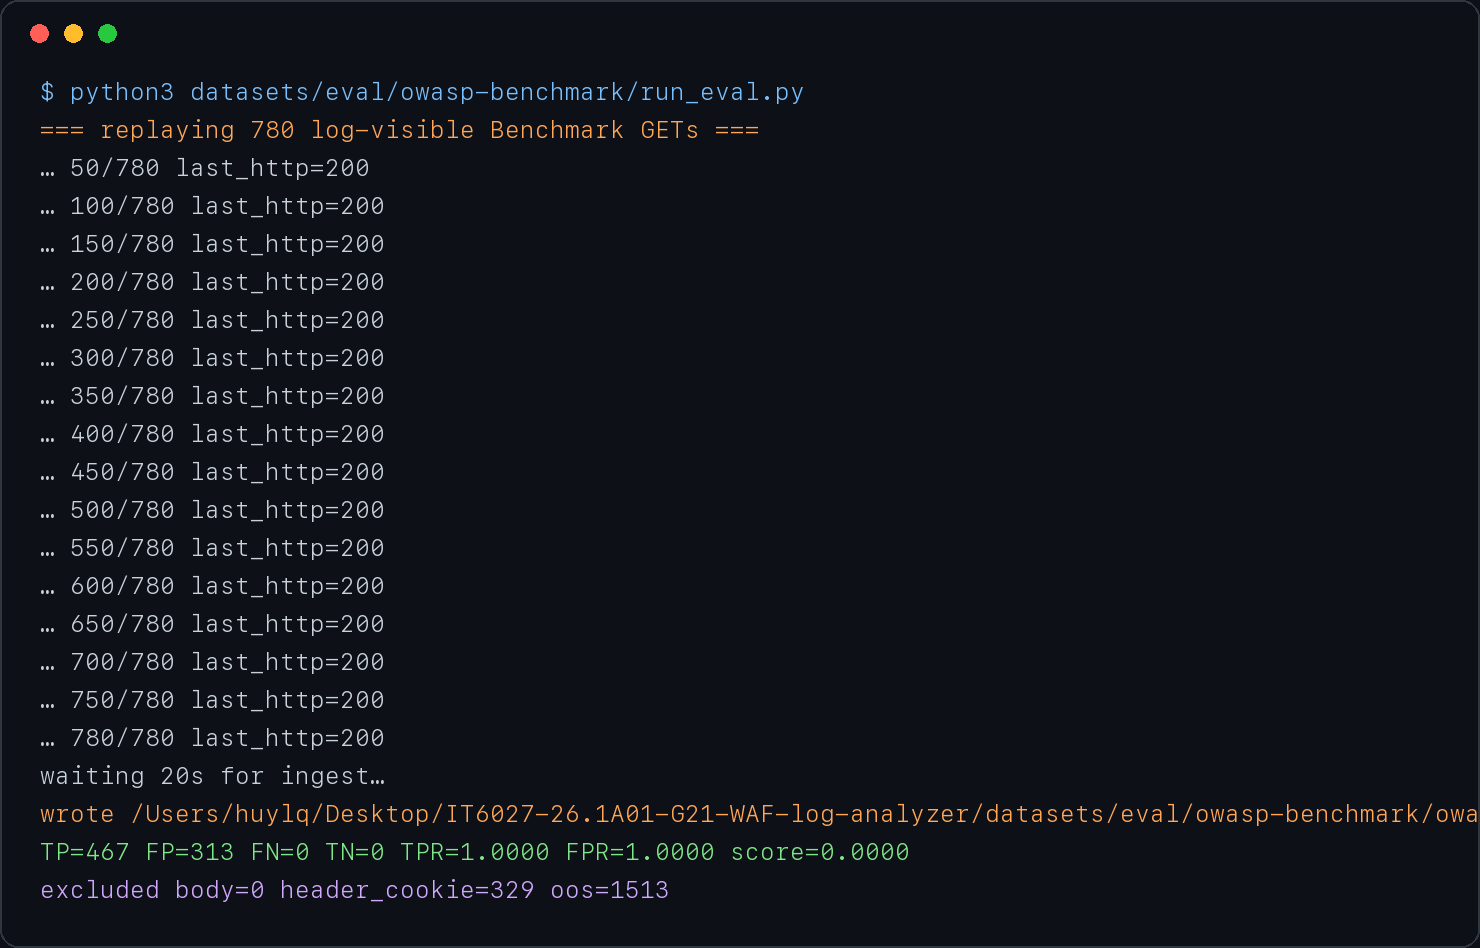
\includegraphics[width=\textwidth]{benchmark-terminal.png}
\caption{Kết quả terminal của lần chạy OWASP Benchmark adaptation trên
lab sạch: 467 TP, 313 FP, 0 FN, 0 TN và score 0.}
\label{fig:benchmark-terminal}
\end{figure}

Ảnh dashboard ở Hình \ref{fig:benchmark-dashboard} là phép kiểm tra chéo
độc lập với file kết quả của runner. Giao diện đọc dữ liệu thật từ REST
API cho thấy 801 WebEvent (780 request Benchmark và 21 request
khởi động/health-check), đúng 780 Alert, 780 Alert mức CRITICAL và một
Incident OPEN do cơ chế \code{IMMEDIATE} gộp cùng ứng dụng/IP. Vì vậy,
con số một Incident không có nghĩa chỉ phát hiện một request; quan hệ
780 Alert--một Incident là kết quả của correlation key
\((appId,clientIp)\) trong cửa sổ thời gian.

\begin{figure}[H]
\centering
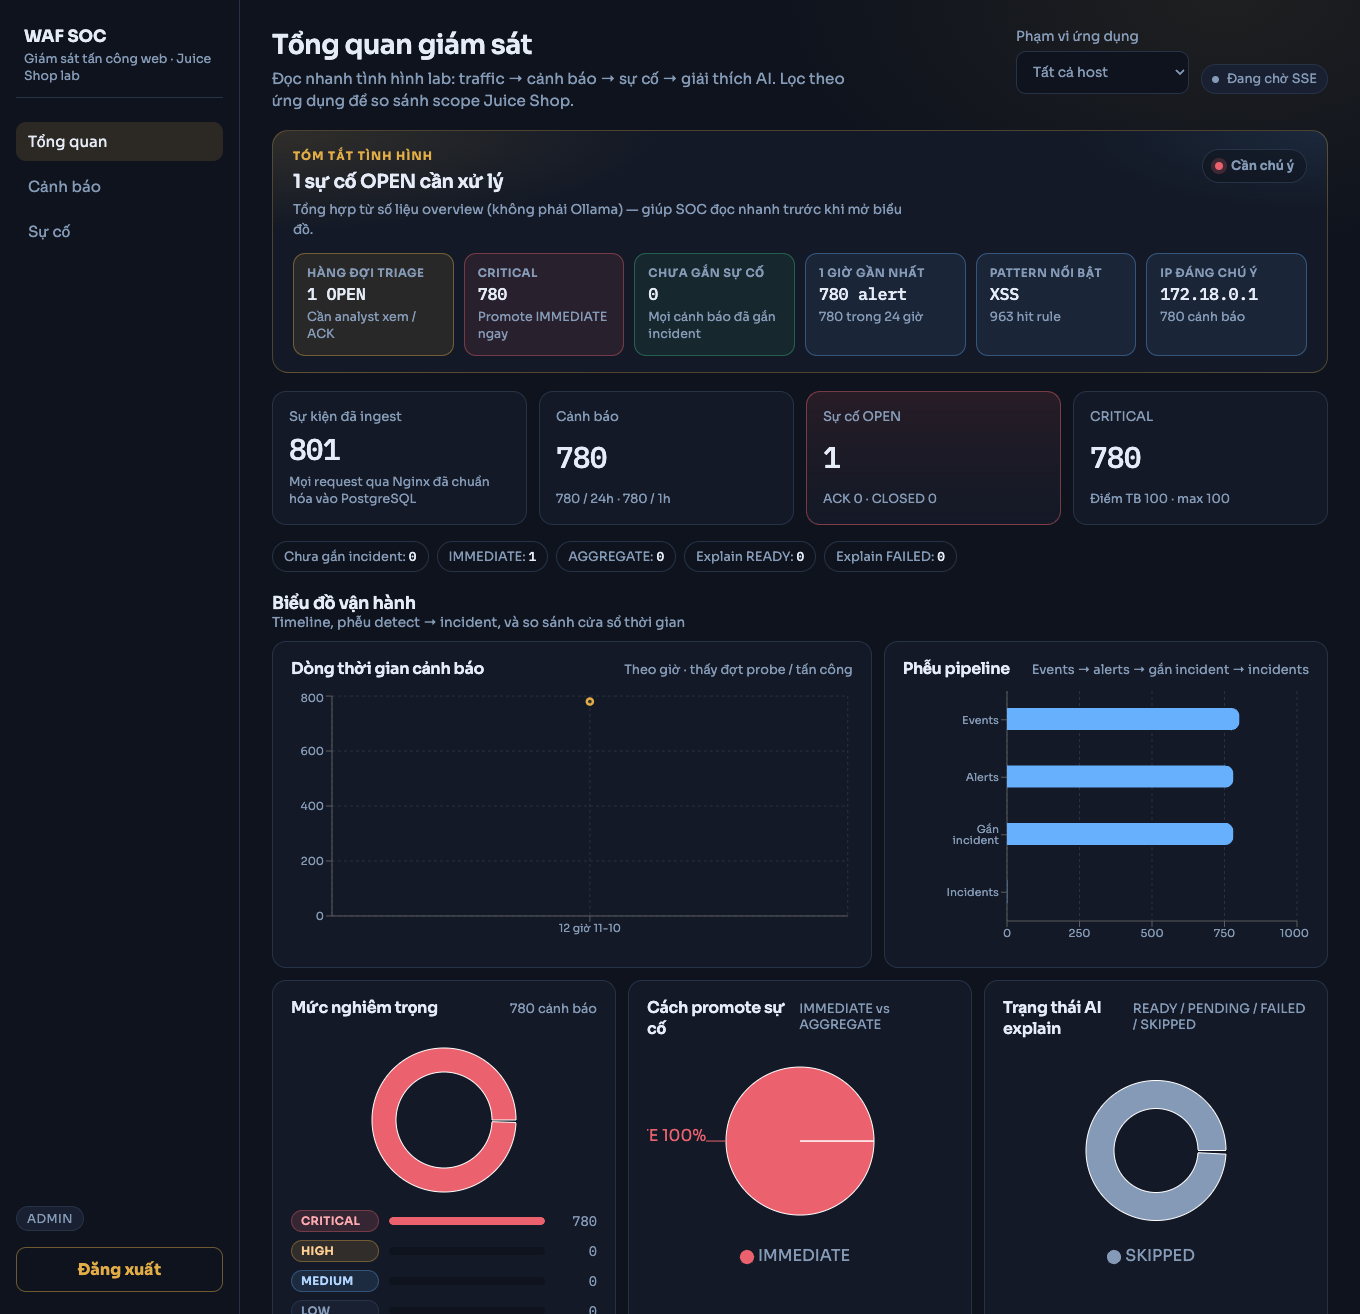
\includegraphics[width=0.98\textwidth]{benchmark-dashboard.png}
\caption{Dashboard SOC sau lần replay: 801 event được ingest, 780 Alert,
780 CRITICAL và một Incident được tương quan.}
\label{fig:benchmark-dashboard}
\end{figure}

Hình \ref{fig:benchmark-alerts} phóng to lớp bằng chứng Alert. Màn hình
hiển thị 780/780 bản ghi, điểm trung bình 100 và các test id
\code{BenchmarkTest0265x} còn nguyên trong path/query, cho phép truy vết
từ case đầu vào đến WebEvent, Alert và Incident. Các ảnh chỉ là bằng
chứng quan sát; artifact có thể kiểm tra bằng máy vẫn là
\code{owasp-benchmark.md} và \code{scored-cases.csv}.

\begin{figure}[H]
\centering
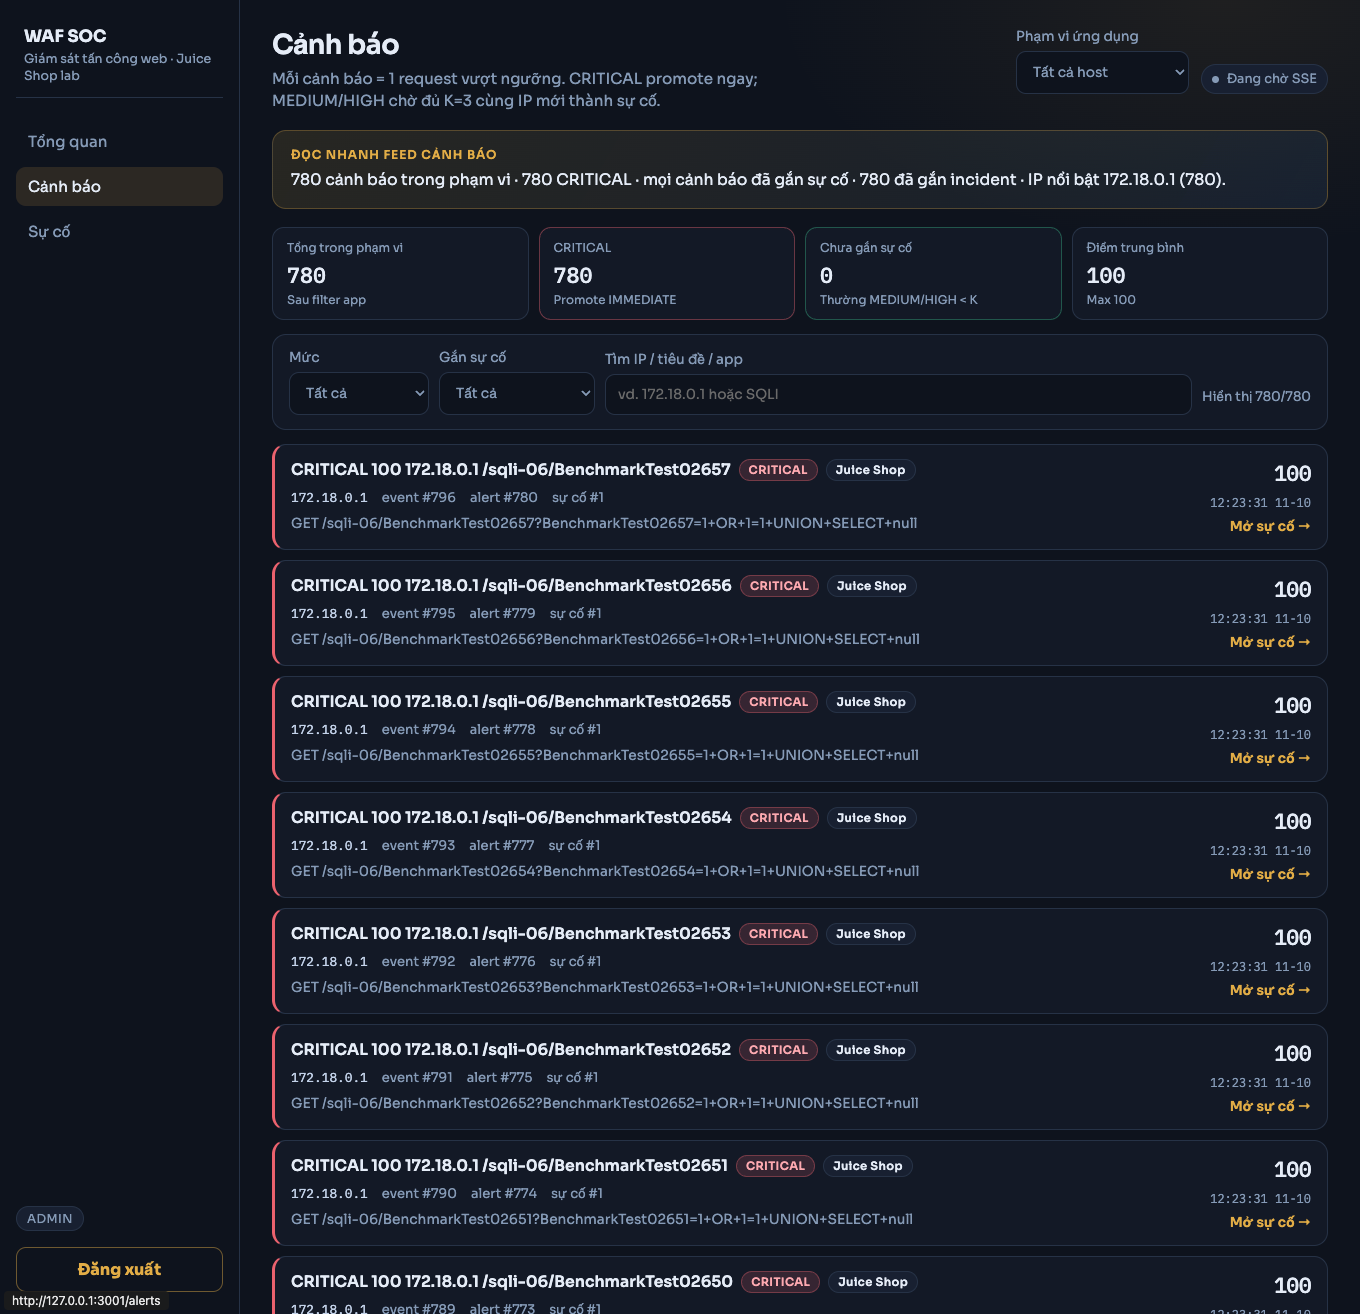
\includegraphics[width=0.98\textwidth]{benchmark-alerts.png}
\caption{Danh sách Alert thật sau replay, thể hiện test id, payload SQLi,
event id, alert id, incident id, severity và risk score.}
\label{fig:benchmark-alerts}
\end{figure}

\subsubsection{Diễn giải phép tính score bằng số cụ thể}

Trong 780 case được chấm có 467 nhãn \code{true} và 313 nhãn
\code{false}. Production rules tạo Alert cho cả 780 request:
\[
\begin{aligned}
TPR &= \frac{467}{467+0}=1,000,\\
FPR &= \frac{313}{313+0}=1,000,\\
Score &= 1,000-1,000=0,000.
\end{aligned}
\]

Không có FN vì toàn bộ 467 case nhãn true đều nhận Alert. Không có TN vì
toàn bộ 313 case nhãn false cũng nhận Alert. Kết quả theo category có
cùng hình dạng: mọi request đều positive, nên từng category đều có
\(TPR=FPR=1\) và score 0.

Nếu tính thêm metric không phải score chính thức, precision của verdict
theo nhãn Benchmark là:
\[
Precision=\frac{467}{467+313}=0,5987,
\]
accuracy cũng bằng \(467/780=0,5987\), còn balanced accuracy là
\((TPR+TNR)/2=(1+0)/2=0,5\). Accuracy 59,87\% chỉ phản ánh tỷ lệ case
vulnerable trong subset khi classifier luôn báo positive; nó không cho
thấy khả năng phân biệt.

\subsubsection{Tại sao detector báo cả case \code{false}?}

Nhãn \code{false} của Benchmark không có nghĩa request benign. Nó có
nghĩa implementation của test case xử lý input an toàn và không tạo lỗ
hổng. Runner vẫn gửi chuỗi như \code{UNION SELECT}, tag script hoặc
\code{../../}. Bộ phân tích access log được thiết kế để nhận ra
\emph{attack attempt}; nó không có static/data-flow knowledge để biết
servlet đích parameterize SQL, encode output hay canonicalize path.

Do đó:
\begin{itemize}
  \item Với SOC, cảnh báo một attack attempt nhắm vào endpoint đã vá vẫn
  có thể hữu ích cho threat hunting.
  \item Với OWASP Benchmark, cùng cảnh báo đó là FP vì câu hỏi đánh giá là
  ``code có vulnerable không?''.
  \item Score 0 ở đây chứng minh detector không phân loại
  \emph{vulnerable-code state}; nó không phủ định việc detector nhận ra
  780/780 request có payload tấn công.
\end{itemize}

Đây là lệch ontology giữa hai bài toán, không chỉ là threshold sai.
Giảm threshold không tạo TN; tăng threshold đủ cao có thể biến mọi verdict
thành negative, khi đó TPR và FPR cùng 0 và score vẫn 0. Muốn score dương,
công cụ phải đưa ra tỷ lệ positive cao hơn trên case truly vulnerable so
với case safe, điều mà signature chỉ nhìn request không đủ thông tin để
thực hiện.

\subsubsection{Giá trị và giới hạn của thí nghiệm}

Thí nghiệm vẫn có giá trị ở ba điểm: kiểm tra pipeline chịu được 780
request có định danh; xác nhận payload mạnh đi qua Nginx--Kafka--rule
engine tới Alert; và minh họa rủi ro dùng sai ground truth. Tuy nhiên
không được dùng kết quả để tuyên bố hệ thống ``đạt'' hoặc ``trượt'' OWASP
Benchmark theo nghĩa chính thức, vì:
\begin{itemize}
  \item BenchmarkJava WAR không được deploy; code mang nhãn không xử lý
  request replay.
  \item Payload là fixed family payload, không phải request/payload gốc
  riêng của từng Benchmark case.
  \item Chỉ 28,47\% corpus được chấm và chỉ ba category.
  \item Các case \code{false} không nhận benign control; tất cả request
  đều chứa attack syntax.
  \item Scoring lấy Alert sau threshold 60, không đo riêng rule hit;
  Event--case được ghép bằng test name và có thể bị ảnh hưởng nếu lab
  không sạch.
\end{itemize}

\subsubsection{Giao thức cải tiến đề xuất}

Có hai phép đánh giá khác nhau cần tách:
\begin{enumerate}
  \item \textbf{Đánh giá chuẩn Benchmark:} deploy BenchmarkJava, phát
  đúng request từng test case, rồi dùng một công cụ có nhiệm vụ kết luận
  endpoint vulnerable/safe. Khi đó nhãn expected results và verdict cùng
  trả lời một câu hỏi.
  \item \textbf{Đánh giá attack-attempt detector:} bỏ nhãn
  vulnerable-code; gắn mọi request chứa fixed attack payload là positive,
  đồng thời gửi benign control tương ứng tới từng route để đo FP. Có thể
  tạo 780 attack + 780 benign request, khóa trước payload, threshold và
  quy tắc ghép event. Giao thức này phù hợp sản phẩm hiện tại hơn nhưng
  không được gọi là official OWASP Benchmark score.
\end{enumerate}

Kết quả external này vì vậy được báo cáo riêng, không gộp với coverage
tầng A hoặc confusion matrix Juice. Juice trả lời ``request gắn nhãn có
tạo Alert không''; Tier A trả lời ``regex có match payload không''; OWASP
Benchmark chính thức trả lời ``công cụ có phân biệt code vulnerable và
safe không''. Ba mẫu số và ba câu hỏi không thể cộng thành một accuracy
duy nhất.

\subsection{Độ trễ, kiểm thử mã và giá trị nội tại}

Probe latency SQLi đo thời gian request--Alert API trong nhiều lần chạy
là 11,5--15,1 giây, vượt mục tiêu dưới 5 giây. HTTP chỉ khoảng 0,02
giây; quan sát hiện có quy phần lớn trễ cho Filebeat--Kafka--consumer,
nhưng chưa có tracing thành phần để khẳng định tỷ lệ chính xác. Vì chưa
đo p50/p95 dưới tải, kết quả không đại diện benchmark throughput.

Backend có unit test cho parser, rule engine, scorer, AlertService,
IncidentManager, fan-out và LLM explain. Các test này kiểm tra logic
fixture, không tự động xác nhận artifact đánh giá Python. Giá trị nội tại
bị đe dọa bởi probe do tác giả soạn, ghép event theo query gần đúng, một
lần chạy lab và payload external cố định. Giá trị ngoại tại bị giới hạn
bởi một workload Juice Shop, ba category và không có traffic production.

\section{Thảo luận về quản trị rủi ro}

Giải pháp làm tốt tính truy vết: từ Incident có thể quay về Alert,
WebEvent, hit và rule version. Phân tách Alert--Incident giảm số case SOC
so với quy tắc một cảnh báo là một sự cố. LLM bị cô lập khỏi verdict,
giúp lỗi model không làm mất bằng chứng. Ngược lại, hệ thống hiện chưa có
audit trail đầy đủ cho thay đổi rule/triage, không có rotation refresh
token dù schema đã chuẩn bị, chưa có quản lý người dùng và chưa ký/mã hóa
log bất biến. Đây là khoảng trống quản trị cần ưu tiên trước khi dùng
ngoài lab.

Rủi ro riêng tư phát sinh vì query và user-agent có thể chứa PII hoặc
token. Chính sách 30 ngày chỉ là đề xuất lab; production phải dựa trên
mục đích xử lý, phân loại dữ liệu, yêu cầu pháp lý và khả năng xóa. Quyền
đọc log nên theo least privilege, truy cập phải audit, và dashboard không
được hiển thị secret nguyên dạng.

\section{Kết luận và hướng phát triển}

Đề tài đã hiện thực một chuỗi đầu cuối có thể chạy bằng Compose: thu log,
stream, chuẩn hóa, phát hiện bằng 14 rule, chấm điểm, tạo Alert/Incident,
hiển thị SOC và giải thích tùy chọn. Use Case, sequence và ERD đều được
đối chiếu với controller, service và migration hiện tại. Kết quả Juice
cho thấy khả năng phát hiện tốt với XSS/Path Traversal trong tập probe,
nhưng SQLi và latency chưa đạt kỳ vọng. External Benchmark khẳng định
cần chọn metric đúng với câu hỏi an ninh.

Các hướng phát triển ưu tiên là:
\begin{enumerate}
  \item instrument timestamp tại Nginx, Filebeat, Kafka, consumer và SSE
  để tối ưu p95;
  \item bổ sung telemetry body/header theo allow-list, masking và giới
  hạn kích thước;
  \item xây dựng regression corpus và quy trình approval/rollback rule;
  \item bổ sung audit log bất biến, refresh-token rotation, quản lý
  user/app và secret manager;
  \item triển khai feedback false-positive có human approval;
  \item tích hợp WAF inline ở chế độ DetectionOnly trước khi cân nhắc
  block; và đánh giá đa ứng dụng, nhiều lần chạy, dưới tải đồng thời.
\end{enumerate}
Mọi tự động hóa block hoặc điều chỉnh rule phải giữ con người trong vòng
quyết định.

\begin{credits}
\subsubsection{\ackname}
Tác giả sử dụng các dự án mã nguồn mở và bộ dữ liệu được trích dẫn để xây
dựng môi trường thực hành. Các probe chỉ được thực hiện trên OWASP Juice
Shop tự lưu trữ.

\subsubsection{\discintname}
Tác giả không có xung đột lợi ích liên quan đến nội dung báo cáo.
\end{credits}

\begin{thebibliography}{20}

\bibitem{owasptop10}
OWASP Foundation: OWASP Top 10: The Ten Most Critical Web Application
Security Risks (2021), \url{https://owasp.org/Top10/}, last accessed
2026/10/11

\bibitem{owaspsqli}
OWASP Foundation: SQL Injection,
\url{https://owasp.org/www-community/attacks/SQL_Injection}, last
accessed 2026/10/11

\bibitem{owaspxss}
OWASP Foundation: Cross Site Scripting (XSS),
\url{https://owasp.org/www-community/attacks/xss/}, last accessed
2026/10/11

\bibitem{owasppath}
OWASP Foundation: Path Traversal,
\url{https://owasp.org/www-community/attacks/Path_Traversal}, last
accessed 2026/10/11

\bibitem{csic}
Information Security Institute, CSIC: HTTP DATASET CSIC 2010,
\url{https://www.isi.csic.es/dataset/}, last accessed 2026/10/11

\bibitem{httpParams}
Morzeux: HttpParamsDataset,
\url{https://github.com/Morzeux/HttpParamsDataset}, last accessed
2026/10/11

\bibitem{modsecurity}
OWASP Foundation: OWASP ModSecurity Core Rule Set,
\url{https://owasp.org/www-project-modsecurity-core-rule-set/}, last
accessed 2026/10/11

\bibitem{wafbooster}
Wu, Y., et al.: WAFBooster: Automatic Boosting of Web Application
Firewalls. arXiv preprint arXiv:2501.14008 (2025)

\bibitem{genxss}
Babaey, M., Ravindran, B.: GenXSS: An AI-driven Framework for Automated
XSS Payload Generation and WAF Rule Creation. arXiv preprint
arXiv:2504.08176 (2025)

\bibitem{modseclearn}
Scano, G., et al.: ModSec-Learn: Boosting ModSecurity with Machine
Learning. arXiv preprint arXiv:2406.13547 (2024),
\url{https://arxiv.org/abs/2406.13547}

\bibitem{rulecache}
Chen, Y., et al.: RuleCache: Accelerating Web Application Firewalls by
On-line Learning Traffic Patterns. In: IEEE International Conference on
Web Services (ICWS), pp. 222--231 (2022).
\doi{10.1109/ICWS55610.2022.00041}

\bibitem{kafka}
Kreps, J., Narkhede, N., Rao, J.: Kafka: A Distributed Messaging System
for Log Processing. In: Proceedings of the NetDB, pp. 1--7 (2011)

\bibitem{juice}
OWASP Foundation: OWASP Juice Shop,
\url{https://owasp.org/www-project-juice-shop/}, last accessed 2026/10/11

\bibitem{owaspbenchmark}
OWASP Foundation: OWASP Benchmark,
\url{https://owasp.org/www-project-benchmark/}, last accessed 2026/10/11

\bibitem{nistcsf}
Pascoe, C., Quinn, S., Scarfone, K.: The NIST Cybersecurity Framework
(CSF) 2.0. NIST CSWP 29, National Institute of Standards and Technology
(2024). \doi{10.6028/NIST.CSWP.29}

\bibitem{iso27001}
International Organization for Standardization: ISO/IEC 27001:2022
Information security, cybersecurity and privacy protection ---
Information security management systems --- Requirements. ISO, Geneva
(2022)

\bibitem{spring}
VMware: Spring Security Reference,
\url{https://docs.spring.io/spring-security/reference/}, last accessed
2026/10/11

\bibitem{filebeat}
Elastic: Filebeat Reference,
\url{https://www.elastic.co/guide/en/beats/filebeat/current/}, last
accessed 2026/10/11

\bibitem{nginx}
F5, Inc.: NGINX Documentation,
\url{https://nginx.org/en/docs/}, last accessed 2026/10/11

\bibitem{postgresql}
PostgreSQL Global Development Group: PostgreSQL 16 Documentation,
\url{https://www.postgresql.org/docs/16/}, last accessed 2026/10/11

\end{thebibliography}
\end{document}
